%%%%%%%%%%%%%%%%%%%%%%%%%%%%%%%%%%%%%%%%%%%%%%%%%%%%%%%%%%%%
% UNCOMMENT THE LINE BELOW TO VIEW COMMENTS
% \def\DraftVersion {}
%%%%%%%%%%%%%%%%%%%%%%%%%%%%%%%%%%%%%%%%%%%%%%%%%%%%%%%%%%%%

\documentclass[a4paper,11pt]{report}

% \sloppy

%%%%%%%%%%%%%%%%%%%%%%%%%%%%%%%%%%%%%%%%%%%%%%%%%%%%%%%%%%%%
% PACKAGES
%%%%%%%%%%%%%%%%%%%%%%%%%%%%%%%%%%%%%%%%%%%%%%%%%%%%%%%%%%%%
\usepackage[utf8x]{inputenc}

\usepackage[english]{babel} % francais,

\usepackage{fourier}
\usepackage{eulervm}

\usepackage{amsmath,amssymb,amsthm,url}
\usepackage{amsfonts}

% \usepackage{caption}
\usepackage{subcaption}
% \usepackage{marginnote}

% \usepackage[pdftex]{graphicx,color}
\usepackage[pdftex,
		colorlinks=true,
		pagebackref=true,
		citecolor=darkgreen,
		linkcolor=darkblue,
		urlcolor=darkpurple,
	]{hyperref}

\hypersetup{
	pdftitle={IMITATOR User Manual},
	pdfauthor={\'Etienne Andr\'e}%
}


% BEGIN Watermarking
\ifdefined\DraftVersion
	\usepackage{draftwatermark}
	\SetWatermarkText{draft}
	\SetWatermarkScale{2}
	\SetWatermarkColor[gray]{0.9}
\fi
% END Watermarking


%%%%%%%%%%%%%%%%%%%%%%%%%%%%%%%%%%%%%%%%%%%%%%%%%%%%%%%%%%%%
% TIKZ
%%%%%%%%%%%%%%%%%%%%%%%%%%%%%%%%%%%%%%%%%%%%%%%%%%%%%%%%%%%%
\usepackage{pgf}
\usepackage{tikz}
\usetikzlibrary{arrows,automata,decorations.pathmorphing}
% Couleurs

\definecolor{darkblue}{rgb}{0, 0, 0.7}
\definecolor{darkgreen}{rgb}{0, 0.5, 0}
\definecolor{darkpurple}{rgb}{0.7, 0, 0.7}


\definecolor{turquoise}{rgb}{0 0.41 0.41}
\definecolor{rouge}{rgb}{0.79 0.0 0.1}
\definecolor{vert}{rgb}{0.15 0.4 0.1}
\definecolor{mauve}{rgb}{0.6 0.4 0.8}
\definecolor{violet}{rgb}{0.58 0. 0.41}
\definecolor{orange}{rgb}{0.8 0.4 0.2}
\definecolor{bleu}{rgb}{0.39, 0.58, 0.93}
\definecolor{gris}{rgb}{0.6,0.6,0.6}
\definecolor{grisfonce}{rgb}{0.4,0.4,0.4}
% Jeu de couleurs pales
\definecolor{cpale1}{rgb}{1, 0.3, 0.3}
\definecolor{cpale2}{rgb}{0.3, 1, 0.3}
\definecolor{cpale3}{rgb}{0.3, 0.3, 1}
\definecolor{cpale4}{rgb}{1, 0.3, 1}
\definecolor{cpale5}{rgb}{1, 1, 0.3}
\definecolor{cpale6}{rgb}{0.3, 1, 1}
\definecolor{cpale7}{rgb}{0.9, 0.6, 0.2}
\definecolor{cpale8}{rgb}{0.7, 0.4, 1}
\definecolor{cpale9}{rgb}{0.5, 1, 0.75}
\definecolor{cpale10}{rgb}{0.8, 0.7, 0.6}
\definecolor{cpale11}{rgb}{0.6, 0.7, 0.8}
\definecolor{cpale12}{rgb}{0.2, 0.5, 0.9}
\definecolor{cpale13}{rgb}{0.5, 0.9, 0.2}
\definecolor{cpale14}{rgb}{0.9, 0.2, 0.5}
\definecolor{cpale15}{rgb}{0.7, 0.7, 0.7}
\definecolor{cpale16}{rgb}{0.8, 0.8, 0.5}


%%%%%%%%%%%%%%%%%%%%%%%%%%%%%%%%%%%%%%%%%%%%%%%%%%%%%%%%%%%%
% CLEVER REFERENCES
%%%%%%%%%%%%%%%%%%%%%%%%%%%%%%%%%%%%%%%%%%%%%%%%%%%%%%%%%%%%
\usepackage[capitalise,english,nameinlink]{cleveref} % load after algorithm2e and hyperref
% \crefname{line}{\text{line}}{\text{lines}} % to remove the capital


%%%%%%%%%%%%%%%%%%%%%%%%%%%%%%%%%%%%%%%%%%%%%%%%%%%%%%%%%%%%
% CONSTANTS
%%%%%%%%%%%%%%%%%%%%%%%%%%%%%%%%%%%%%%%%%%%%%%%%%%%%%%%%%%%%
%-%-%-%-%-%-%-%-%-%-%-%-%-%-%-%-%-%-%-%-%-%-%-%-%-%-%-%-%-%
% MATHS
%-%-%-%-%-%-%-%-%-%-%-%-%-%-%-%-%-%-%-%-%-%-%-%-%-%-%-%-%-%
% Variables
\def\init{\ensuremath{\textsf{init}}} % \xspace
\newcommand{\A}{\mathcal{A}}
\newcommand{\Action}{\ensuremath{\Sigma}}
\newcommand{\action}{a}
\newcommand{\C}{C}
\newcommand{\Cinit}{\C_\init} % initial constraint
\newcommand{\Clock}{X} % set of clocks
\newcommand{\ClockCard}{H} % cardinality of clocks
\newcommand{\clock}{x} % clock
\newcommand{\clockval}{w} % clock valuation
\newcommand{\Cupdates}{\Clock_\mathsf{up}}
\newcommand{\Dupdates}{\DVar_\mathsf{up}}
\newcommand{\dval}{\ensuremath{\delta}} % discrete variable
\newcommand{\DVar}{D} % set of discrete variables
\newcommand{\dvar}{d} % discrete variable
\newcommand{\DVarCard}{J} % cardinality of discrete variables
% \newcommand{\DVarinit}{\DVar_\init} % discrete variable
\newcommand{\edge}{e}
\newcommand{\guard}{g}
\newcommand{\invariant}{I}
\newcommand{\LConstraint}{\mathcal{LC}} % (#1)% set of all constraints over some set
\newcommand{\LConstraintD}{\LConstraint(\DVar)}
\newcommand{\LConstraintXP}{\LConstraint(\Clock \cup \Param)}
\newcommand{\LConstraintXPD}{\LConstraint(\Clock \cup \Param \cup \DVar)}
\newcommand{\lterm}{\mathit{lt}}
\newcommand{\LTerm}{\mathcal{LT}} % (#1)% set of all linear terms over some set
\newcommand{\LTermD}{\LTerm(\DVar)}
\newcommand{\LTermXPD}{\LTerm(\Clock \cup \Param \cup \DVar)}
\newcommand{\loc}{l} % location
\newcommand{\locinit}{\loc_\init}
\newcommand{\Loc}{L} % set of locations
\newcommand{\Param}{P} % set of parameters
\newcommand{\param}{p} % parameter
\newcommand{\ParamCard}{M} % number of parameters
\newcommand{\pval}{v} % parameter valuation
% \newcommand{\resets}{R}
\newcommand{\steps}{ {\rightarrow} }
\newcommand{\stopwatches}{S}
\newcommand{\tuple}[1]{\langle#1\rangle}
\newcommand{\unobs}{\ensuremath{\epsilon}}
\newcommand{\Var}{\mathit{Var}} % set of variables
\newcommand{\var}{\mathit{z}} % variable
\newcommand{\VarCard}{N} % cardinality of variables % TODO: conflict

% Ensembles
\newcommand{\grandb}{{\mathbb B}}
\newcommand{\grandn}{{\mathbb N}}
\newcommand{\grandq}{{\mathbb Q}}
\newcommand{\grandqplus}{{\mathbb Q}_{\geq 0}}
\newcommand{\grandr}{{\mathbb R}}
\newcommand{\grandrplus}{\grandr_{\geq 0}}
\newcommand{\grandz}{{\mathbb Z}}

% Unites
\newcommand{\micros}{\mathit{\mu s}}
\newcommand{\nanos}{ns}

% Noms
\newcommand{\tiling}{\mathit{Tiling}}
% \newcommand{\true}{\mathbf{true}}
\newcommand{\Ko}{K}
\newcommand{\pio}{\pi_0}
\newcommand{\piprime}{\pi}
\newcommand{\To}{T_0}
\newcommand{\Tprime}{T}

% Symboles
\newcommand{\emptystring}{$\epsilon$}
\newcommand{\fleche}[1]{\stackrel{#1}{\rightarrow}}
\newcommand{\Fleche}[1]{\stackrel{#1}{\Rightarrow}}
% \newcommand{\steps}[0]{ {\rightarrow} }

% Booleens
\newcommand{\false}{{\tt false}}
\newcommand{\true}{{\tt true}}

% PARAMETRES RCP
\newcommand{\rcpFMax}{\mathit{rc\_fast\_max}}
\newcommand{\rcpFMin}{\mathit{rc\_fast\_min}}
\newcommand{\rcpSMax}{\mathit{rc\_slow\_max}}
\newcommand{\rcpSMin}{\mathit{rc\_slow\_min}}
\newcommand{\rcpD}{\mathit{delay}}

%-%-%-%-%-%-%-%-%-%-%-%-%-%-%-%-%-%-%-%-%-%-%-%-%-%-%-%-%-%
% ALGORITHMES
%-%-%-%-%-%-%-%-%-%-%-%-%-%-%-%-%-%-%-%-%-%-%-%-%-%-%-%-%-%
% Algorithmes PTA
\newcommand{\BC}{\ensuremath{\mathsf{BC}}}
\newcommand{\EFsynth}{\ensuremath{\mathsf{EFsynth}}}
\newcommand{\IM}{\ensuremath{\mathsf{IM}}}
\newcommand{\PDFC}{\ensuremath{\mathsf{PDFC}}}
\newcommand{\PRP}{\ensuremath{\mathsf{PRP}}}
\newcommand{\PRPC}{\ensuremath{\mathsf{PRPC}}}


%-%-%-%-%-%-%-%-%-%-%-%-%-%-%-%-%-%-%-%-%-%-%-%-%-%-%-%-%-%
% CONSTANTES DE CHAINES
%-%-%-%-%-%-%-%-%-%-%-%-%-%-%-%-%-%-%-%-%-%-%-%-%-%-%-%-%-%

% Outils
% \newcommand{\apron}{\textsc{Apron}}
\newcommand{\CosyVerif}{\emph{CosyVerif}}
\newcommand{\gdot}{\texttt{dot}}
\newcommand{\graphviz}{Graphviz}
\newcommand{\hytech}{{\sc HyTech}}
% \newcommand{\imitator}{\textsc{Imitator}}
\newcommand{\imitator}{\textsf{IMITATOR}}
\newcommand{\imitatorExec}{\code{imitator}}
\newcommand{\IPTA}{IPTA}
\newcommand{\NIPTA}{NIPTA}
\newcommand{\ocaml}{OCaml}
\newcommand{\pat}{PAT}
\newcommand{\phaver}{PHAVer}
% \newcommand{\polka}{NewPolka}
% \newcommand{\prism}{\textsc{Prism}}
% \newcommand{\red}{RED}
\newcommand{\uppaal}{\textsc{Uppaal}}

\newcommand{\binimitator}{./imitator}


% Current version
\newcommand{\imitatorversion}{2.8}
\newcommand{\imitatorversionname}{Butter Ham}


%%%%%%%%%%%%%%%%%%%%%%%%%%%%%%%%%%%%%%%%%%%%%%%%%%%%%%%%%%%%
% THEOREMS
%%%%%%%%%%%%%%%%%%%%%%%%%%%%%%%%%%%%%%%%%%%%%%%%%%%%%%%%%%%%
\newtheorem{definition}{Definition}
\newtheorem{remark}{Remark}
\newtheorem{hint}{Hint}


%%%%%%%%%%%%%%%%%%%%%%%%%%%%%%%%%%%%%%%%%%%%%%%%%%%%%%%%%%%%
% FORMATING
%%%%%%%%%%%%%%%%%%%%%%%%%%%%%%%%%%%%%%%%%%%%%%%%%%%%%%%%%%%%

\hyphenation{IMITATOR}
\hyphenation{Uppaal}

% \newcommand{\paragraphe}[1]{\paragraph{#1.}}

% Non terminal in a grammar
\newcommand{\nt}[1]{$\langle$\emph{#1}$\rangle$}
% Rule name in a grammar
\newcommand{\regleGrammaire}[1]{\bigskip \noindent \nt{#1} :: \\}
% Not taken into account in the grammar
\newcommand{\npec}[1]{\textcolor{green!50!black}{#1}}

\newcommand{\probleme}[2]{
	\medskip
	\noindent
	\fbox{
		\begin{minipage}{0.95\textwidth}
		\textbf{#1}
		
		#2
		\end{minipage}
	}
	
	\medskip
}

% \newcommand{\commentaire}[1]{\textcolor{red}{\textbf{$\Leftarrow$  #1 $\Rightarrow$}}} % commentaire dans un paragraphe
% \newcommand{\commentaire}[1]{}


% Code integre au texte
\newcommand{\code}[1]{\textbf{\texttt{#1}}}


\definecolor{imicolor}{rgb}{0, .4, .4}
\newcommand{\styleIMI}[1]{\textcolor{imicolor}{\texttt{#1}}}

\definecolor{optioncolor}{rgb}{.4, 0, .4}
\newcommand{\styleOption}[1]{\textcolor{optioncolor}{\texttt{#1}}}
\newcommand{\styleOptionValue}[1]{\textcolor{optioncolor}{\texttt{#1}}}

\definecolor{pathcolor}{rgb}{1, .5, 0}
\newcommand{\stylePath}[1]{\textcolor{pathcolor}{\texttt{#1}}}

\definecolor{filecontentcolor}{rgb}{.1, .4, .2}
\newcommand{\styleFileContent}[1]{\textcolor{filecontentcolor}{\texttt{#1}}}

\newcommand{\GitHubIMI}{GitHub} % TODO : URL

\newcommand{\styleCommand}[1]{
	\medskip
	
	% \mbox{}\hspace{.5cm}
	\noindent\fcolorbox{white}{black!90}{
		\textcolor{yellow!30}{\$\ \ \texttt{#1}}
	}
	
	\medskip

}

\newcommand{\styleTerminalOutput}[1]{
	\medskip
	
	% \mbox{}\hspace{.5cm}
	\noindent\fcolorbox{white}{black!90}{
	\begin{minipage}{.97\textwidth}
		\textcolor{yellow!30}{\texttt{#1}}
	\end{minipage}
	}
	
	\medskip

}



%%%%%%%%%%%%%%%%%%%%%%%%%%%%%%%%%%%%%%%%%%%%%%%%%%%%%%%%%%%%
% I.E. / E.G. / W.R.T.
%%%%%%%%%%%%%%%%%%%%%%%%%%%%%%%%%%%%%%%%%%%%%%%%%%%%%%%%%%%%

% Helps to spot the places where macros are NOT used
\ifdefined \DraftVersion
 	\definecolor{colorok}{RGB}{80,80,150}
\else
	\definecolor{colorok}{RGB}{0,0,0}
\fi

% \newcommand{\eg}{\textcolor{colorok}{\textit{e.g.}}\xspace}
% \newcommand{\ie}{\textcolor{colorok}{\textit{i.e.}}\xspace}
% \newcommand{\wrt}{\textcolor{colorok}{w.r.t.}\xspace}
\newcommand{\adhoc}{\textcolor{colorok}{\textit{ad-hoc}\@}}
\newcommand{\eg}{\textcolor{colorok}{\textit{e.g.},\@}}
\newcommand{\ie}{\textcolor{colorok}{\textit{i.e.},\@}}
\newcommand{\wrt}{\textcolor{colorok}{w.r.t.}\@}





%%%%%%%%%%%%%%%%%%%%%%%%%%%%%%%%%%%%%%%%%%%%%%%%%%%%%%%%%%%%
% IMITATOR FILES
%%%%%%%%%%%%%%%%%%%%%%%%%%%%%%%%%%%%%%%%%%%%%%%%%%%%%%%%%%%%
\usepackage{listings}
\newcommand{\IncludeIMIfile}[1]{
	\lstset{language=Imitator}
	\lstinputlisting[
		basicstyle=\footnotesize,
		breaklines=true,
		breakatwhitespace=true,
		columns=fixed,
		numbers=left,
		frame=single,
		numberstyle=\tiny,
		tabsize=4,
% 		title=\lstname
	]{#1}
}

\lstdefinelanguage{Imitator}{
	morekeywords={
		and, automaton, clock, constant, discrete, do, end, endreach, False, forward, from, goto, if, in, init, initially, loc, locations, not, or, parameter, print, property, reach, region, unreachable, urgent, sync, synclabs, True, var, wait, when, while
	},
	sensitive=false,
% 	morecomment=[l][\color{gray}]{--},
	morecomment=[s][keywordstyle]{"}{"},
% 	morecomment=[s]{/*}{*/},
	morecomment=[s][\color{gray!50!blue}]{(*}{*)},
}


%%%%%%%%%%%%%%%%%%%%%%%%%%%%%%%%%%%%%%%%%%%%%%%%%%%%%%%%%%%%
%%%%%%%%%%%%%%%%%%%%%%%%%%%%%%%%%%%%%%%%%%%%%%%%%%%%%%%%%%%%
%%%%%%%%%%%%%%%%%%%%%%%%%%%%%%%%%%%%%%%%%%%%%%%%%%%%%%%%%%%%

% Title Page
\title{IMITATOR User Manual}
\author{Étienne André}
% \date{}

\begin{document}
% \maketitle

\sloppy


%%%%%%%%%%%%%%%%%%%%%%%%%%%%%%%%%%%%%%%%%%%%%%%%%%%%%%%%%%%%
\thispagestyle{empty}

\mbox{}

\vspace{2cm}

\begin{center}
	{\Huge \bfseries IMITATOR User Manual}

	\vspace{2cm}

	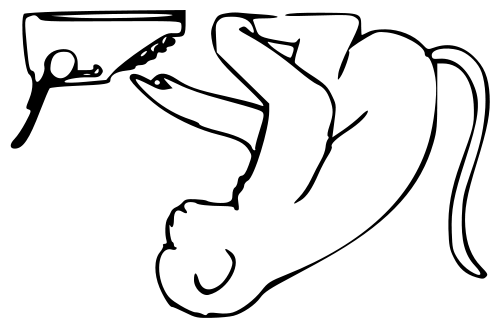
\includegraphics[width=0.50\textwidth]{../logos/imitator-500.png}

	\vspace{2.5cm}
	
	{\Large Version \imitatorversion{} (\imitatorversionname{})}
	
	\medskip
	
	
\includegraphics[height=0.15\textwidth]{../logos/logo2-300.png}
% 	
	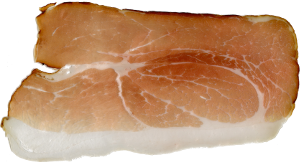
\includegraphics[height=0.15\textwidth]{../logos/logo2-8-300.png}

\end{center}

\vspace{1.5cm}

{\small \hfill{}Build \input{../build_number.txt}}

{\small \hfill{}\today{}}

\vspace{2cm}

\begin{center}
 	{\Large \url{www.imitator.fr}}
 	
\end{center}
\hfill
\includegraphics[width=.15\textwidth]{images/CC-BY-SA_500.png}



%%%%%%%%%%%%%%%%%%%%%%%%%%%%%%%%%%%%%%%%%%%%%%%%%%%%%%%%%%%%

\newpage

%%%%%%%%%%%%%%%%%%%%%%%%%%%%%%%%%%%%%%%%%%%%%%%%%%%%%%%%%%%%
\tableofcontents
\addcontentsline{toc}{section}{Table of contents}
%%%%%%%%%%%%%%%%%%%%%%%%%%%%%%%%%%%%%%%%%%%%%%%%%%%%%%%%%%%%

\newpage

% \pagestyle{fancyplain}
% \lhead{\fancyplain{}{\imitator{} \imitatorversion{} User Manual}}



%%%%%%%%%%%%%%%%%%%%%%%%%%%%%%%%%%%%%%%%%%%%%%%%%%%%%%%%%%%%
%%%%%%%%%%%%%%%%%%%%%%%%%%%%%%%%%%%%%%%%%%%%%%%%%%%%%%%%%%%%
\chapter{Introduction}
%%%%%%%%%%%%%%%%%%%%%%%%%%%%%%%%%%%%%%%%%%%%%%%%%%%%%%%%%%%%
%%%%%%%%%%%%%%%%%%%%%%%%%%%%%%%%%%%%%%%%%%%%%%%%%%%%%%%%%%%%

\imitator{} is a free, open source software tool to perform automated parameter synthesis for concurrent timed systems~\cite{AFKS12}.
\imitator{} takes as input a network of \imitator{} parametric timed automata (\NIPTA{}): \NIPTA{} are an extension of parametric timed automata~\cite{AHV93}, a well-known formalism to specify and verify models of systems where timing constants can be replaced with parameters, \ie{} unknown constants.

\imitator{} addresses several variants of the following problem:
``given a concurrent timed system, what are the values of the timing constants that guarantee that the model of the system satisfies some property?''
Specifically, \imitator{} implements parametric safety analysis~\cite{AHV93,JLR15}, the inverse method \cite{ACEF09,AM15}, the behavioral cartography~\cite{AF10}, and parametric reachability preservation~\cite{ALNS15}.
Some algorithms can also run distributed on a cluster.
Numerous analysis options are available.

\imitator{} is a command-line only tool, but that can output results in graphical form.
Furthermore, a graphical user interface is available in the \CosyVerif{} platform~\cite{AHHKLLP13}.

\imitator{} was able to verify numerous case studies from the literature and from the industry, such as communication protocols, hardware asynchronous circuits, schedulability problems and various other systems such as coffee machines (probably the most critical systems from a researcher point of view).
Numerous benchmarks are available at \imitator{} Web page~\cite{imitator}.

In this document, we present the input syntax, we formally define the input model of \imitator{}, and we explain how to perform various analyses using the numerous options.


\paragraph{Keywords:} formal verification, model checking, software verification, parameter synthesis


%%%%%%%%%%%%%%%%%%%%%%%%%%%%%%%%%%%%%%%%%%%%%%%%%%%%%%%%%%%%
%%%%%%%%%%%%%%%%%%%%%%%%%%%%%%%%%%%%%%%%%%%%%%%%%%%%%%%%%%%%
\chapter{A Brief Introduction to the Syntax}
%%%%%%%%%%%%%%%%%%%%%%%%%%%%%%%%%%%%%%%%%%%%%%%%%%%%%%%%%%%%
%%%%%%%%%%%%%%%%%%%%%%%%%%%%%%%%%%%%%%%%%%%%%%%%%%%%%%%%%%%%

We first briefly introduce the syntax using a simple example for readers familiar with parametric timed automata, and not interested in subtle details (such as the synchronization model).
A formal (and nearly exhaustive) definition of \imitator{} parametric timed automata (\NIPTA{}) can be found in \cref{section:IPTA}.
The complete syntax is given in \cref{chapter:grammar}.

\paragraph{Generalities}
\imitator{} performs parametric verification of models specified using networks of \imitator{} parametric timed automata (hereafter \NIPTA{}).
An \imitator{} parametric timed automaton (hereafter \IPTA{}) is a variant of parametric automata (as introduced in~\cite{AHV93}).
\IPTA{} and \NIPTA{} are formalized in \cref{section:NIPTA}.

The input syntax of \imitator{} is originally based on the syntax of \hytech{}~\cite{HHW95}, with several improvements.
Actually, all standard \hytech{} files describing only PTA (and not more general systems like linear hybrid automata \cite{achh92}) can be analyzed directly by \imitator{} (sometimes with very minor changes).

Comments are OCaml-like comments starting with \styleIMI{(*} and ending with \styleIMI{*)}.
As in OCaml, comments can be nested.


\paragraph{The Fischer mutual exclusion protocol}
We use as a motivating example one timed version of the Fischer mutual exclusion protocol, coming from the \pat{} model checker~\cite{SLDP09}.
This version of the protocol is neither the most complete, nor the most simple; we just use it here to introduce various aspects of the \imitator{} input syntax.

Fischer mutual exclusion protocol is a protocol that guarantees the mutual exclusion of several processes (here two) that want to access a shared resource (called the critical section).
% We give below an example of a coffee machine interacting with a researching drinking coffee, given using the \imitator{} syntax.
% 	% TODO: point to figure
% 
% \IncludeIMIfile{../examples/Coffee/coffeeDrinker.imi}

\paragraph{Input syntax}
We give below this model using the \imitator{} syntax.
This model is given in graphical form in \cref{figure:fischer}.\footnote{%
	This \LaTeX{} representation, that makes use of the \LaTeX{} TikZ library, was automatically output by \imitator{}, using option \styleOption{-PTA2TikZ}, followed by some manual positioning optimization.
}

\bigskip

%------------------------------------------------------------
\IncludeIMIfile{include/fischerPAT_obs.imi}
%------------------------------------------------------------


% TODO: add graphic representation, describe model, make at least one call (or even one call per algo)


\paragraph{Header}
Let us comment this case model by starting with the header.
First, text in comments gives generalities about the model (author, date, description, etc.).
The form is not normalized, but it could be in the future, so it is strongly advised to follow this form.\footnote{%
	An empty model template with all these comments ready to be filled out (containing also a sample \IPTA{} and its initial definitions) is available at:
	
	\url{https://github.com/etienneandre/imitator/blob/master/benchmarks/model.imi}.
}

\paragraph{Variable declarations}
The variable declarations starts with keyword \styleIMI{var}.

This model contains two clocks: \styleIMI{x1} is process~1's clock, and \styleIMI{x2} is process~2's clock.

This model contains two parameters: \styleIMI{delta} is the parametric duration specifying how long a process is idle at most, whereas \styleIMI{gamma} is the parametric duration specifying the minimum duration between the time a process checks for the availability of the critical section and the time the same process indeed enters the critical section (if it is still available).

Two discrete variables (\ie{} global, integer-valued variables, see \cref{section:discrete}) are used:
	\styleIMI{turn} checks which process is attempting to enter the critical section;
	\styleIMI{counter} records how many processes are in the critical section (this variable will not be used for the verification, but was used in the original \pat{} model, and we choose to keep it).
	% TODO: use it for verification once IMITATOR supports global variables in properties

Finally, a global constant \styleIMI{IDLE} is set to \styleIMI{-1} (just as in the original \pat{} model), and encodes that no process is attempting to enter the critical section.


%------------------------------------------------------------
%%%%%%%%%%%%%%%%%%%%%%%%%%%%%%%%%%%%%%%%%%%%%%%%%%%%%%%%%%%%
 % File automatically generated by IMITATOR
 % Version  : IMITATOR 2.7-beta4 "Butter Guéméné" (build 1205)
 % Model    : 'examples/Fischer/fischerPAT_obs.imi'
 % Generated: Mon Jul 20, 2015 10:34:13
 % 
 % (node positioning not yet supported, you may need to manually edit the file)
 %%%%%%%%%%%%%%%%%%%%%%%%%%%%%%%%%%%%%%%%%%%%%%%%%%%%%%%%%%%%
% \documentclass[a4paper,10pt]{article}
% 
% %%%%%%%%%%%%%%%%%%%%%%%%%%%%%%%%%%%%%%%%%%%%%%%%%%%%%%%%%%%%
% % PACKAGES
% %%%%%%%%%%%%%%%%%%%%%%%%%%%%%%%%%%%%%%%%%%%%%%%%%%%%%%%%%%%%
% \usepackage[T1]{fontenc}
% 
% \usepackage[utf8]{inputenc}
% 
% \usepackage{subcaption}
% 
% % Tikz
% \usepackage{tikz}
% \usetikzlibrary{arrows,automata}
\tikzstyle{every node}=[initial text=]
\tikzstyle{location}=[rectangle, rounded corners, minimum size=12pt, draw=black, inner sep=1.5pt]
\tikzstyle{invariant}=[draw=black, xshift=-1em, inner sep=1pt]
\tikzstyle{urgent}=[dotted, draw=red, very thick]


\definecolor{coloract}{rgb}{0.50, 0.70, 0.30}
\definecolor{colorclock}{rgb}{0.4, 0.4, 1}
\definecolor{colordisc}{rgb}{1, 0, 1}
% \definecolor{colorloc}{rgb}{0.4, 0.4, 0.65}
%%% NOTE: better in black
\definecolor{colorloc}{rgb}{0, 0, 0}
\definecolor{colorparam}{rgb}{1, 0.6, 0.0}

% Set of colors
\definecolor{loccolor1}{rgb}{1, 0.3, 0.3}
\definecolor{loccolor2}{rgb}{0.3, 1, 0.3}
\definecolor{loccolor3}{rgb}{0.3, 0.3, 1}
\definecolor{loccolor4}{rgb}{1, 0.3, 1}
\definecolor{loccolor5}{rgb}{1, 1, 0.3}
\definecolor{loccolor6}{rgb}{0.3, 1, 1}
\definecolor{loccolor7}{rgb}{0.9, 0.6, 0.2}
\definecolor{loccolor8}{rgb}{0.7, 0.4, 1}
\definecolor{loccolor9}{rgb}{0.5, 1, 0.75}
\definecolor{loccolor10}{rgb}{0.8, 0.7, 0.6}
\definecolor{loccolor11}{rgb}{0.6, 0.7, 0.8}
\definecolor{loccolor12}{rgb}{0.2, 0.5, 0.9}
\definecolor{loccolor13}{rgb}{0.5, 0.9, 0.2}
\definecolor{loccolor14}{rgb}{0.9, 0.2, 0.5}
\definecolor{loccolor15}{rgb}{0.7, 0.7, 0.7}
\definecolor{loccolor16}{rgb}{0.8, 0.8, 0.5}

\newcommand{\styleact}[1]{\ensuremath{\textcolor{coloract}{\mathrm{#1}}}}
\newcommand{\styleclock}[1]{\ensuremath{\textcolor{colorclock}{\mathrm{#1}}}}
\newcommand{\styleconst}[1]{\ensuremath{\textcolor{black}{\mathrm{#1}}}} %% ADDED FOR CONSTANTS
\newcommand{\styledisc}[1]{\ensuremath{\textcolor{colordisc}{\mathrm{#1}}}}
\newcommand{\styleloc}[1]{\ensuremath{\textcolor{colorloc}{\mathrm{#1}}}}
\newcommand{\styleparam}[1]{\ensuremath{\textcolor{colorparam}{\mathrm{#1}}}}

% \newcommand{\imitator}{\textsc{Imitator}}

% \title{An IMITATOR model}
% \author{IMITATOR}
% 
% 
% \begin{document}
% 
% \thispagestyle{empty}

\begin{figure}
\newcommand{\ratio}{0.9\textwidth}
	\footnotesize
	\centering
	 
%%%%%%%%%%%%%%%%%%%%%%%%%%%%%%%%%%%%%%%%%%%%%%%%%%%%%%%%%%%%
% automaton proc1
%%%%%%%%%%%%%%%%%%%%%%%%%%%%%%%%%%%%%%%%%%%%%%%%%%%%%%%%%%%%
	\begin{subfigure}[b]{\ratio}
	\centering
	\begin{tikzpicture}[scale=2.5, auto, ->, >=stealth']
 
		\node[location, initial, fill=loccolor1] at (0,0) (idle1) {\styleloc{idle1}};
 
		\node[location, fill=loccolor2] at (-1.5, -1) (active1) {\styleloc{active1}};
		% Invariant of location active1
		\node [invariant,left] at (active1.west) {\begin{tabular}{@{} c @{\ } c@{} }& $ \styleclock{x1} \leq \styleparam{delta}$\\\end{tabular}};
 
		\node[location, fill=loccolor3] at (0,-2) (check1) {\styleloc{check1}};
 
		\node[location, fill=loccolor4] at (0,-3) (access1) {\styleloc{access1}};
 
		\node[location, fill=loccolor5] at (1,-3) (CS1) {\styleloc{CS1}};
 

		\path (idle1) edge[bend right] node[left]{\begin{tabular}{@{} c @{\ } c@{} }
		& $ \styledisc{turn} = \styleconst{IDLE}$\\
		 & $\styleact{try\_1}$\\
		 & $\styleclock{x1}:=0$\\
		\end{tabular}} (active1);
 

		\path (active1)[bend right] edge node[below left]{\begin{tabular}{@{} c @{\ } c@{} }
		 & $\styleact{update\_1}$\\
		 & $\styleclock{x1}:=0$\\
		 & $\styledisc{turn}:=1$\\% 
		\end{tabular}} (check1);
 

		\path (check1) edge node[left]{\begin{tabular}{@{} c @{\ } c@{} }
		& $ \styleclock{x1} \geq \styleparam{gamma}
$\\
		$\land$ & $ \styledisc{turn} = 1$\\
		 & $\styleact{access\_1}$\\
		 & $\styleclock{x1}:=0$\\
		\end{tabular}} (access1);

		%%% NOTE: replace both transitions with '<>'
% 		\path (check1) edge node{\begin{tabular}{@{} c @{\ } c@{} }
% 		& $ \styledisc{turn} > 1
% $\\
% 		$\land$ & $ \styleclock{x1} \geq \styleparam{gamma}$\\
% 		 & $\styleact{no\_access\_1}$\\
% 		 & $\styleclock{x1}:=0$\\
% 		\end{tabular}} (idle1);
% 
% 		\path (check1) edge node{\begin{tabular}{@{} c @{\ } c@{} }
% 		& $ 1 > \styledisc{turn}
% $\\
% 		$\land$ & $ \styleclock{x1} \geq \styleparam{gamma}$\\
% 		 & $\styleact{no\_access\_1}$\\
% 		 & $\styleclock{x1}:=0$\\
% 		\end{tabular}} (idle1);
		\path (check1) edge node{\begin{tabular}{@{} c @{\ } c@{} }
		& $ \styledisc{turn} \neq 1
$\\
		$\land$ & $ \styleclock{x1} \geq \styleparam{gamma}$\\
		 & $\styleact{no\_access\_1}$\\
		 & $\styleclock{x1}:=0$\\
		\end{tabular}} (idle1);
 

		\path (access1) edge node[below]{\begin{tabular}{@{} c @{\ } c@{} }
		 & $\styleact{enter\_1}$\\
		 & $\styledisc{counter}:=\styledisc{counter} + 1$\\% 
		\end{tabular}} (CS1);
 

		\path (CS1) edge[bend right] node[above right]{\begin{tabular}{@{} c @{\ } c@{} }
		 & $\styleact{exit\_1}$\\
		 & $\styleclock{x1}:=0$\\
		 & $\styledisc{counter}:=\styledisc{counter} -1$\\% \n
		 & $\styledisc{turn}:=\styleconst{IDLE}$\\% 
		\end{tabular}} (idle1);
	\end{tikzpicture}
	
	\caption{Process 1}
	\label{pta:proc1}
	\end{subfigure}


% %%%%%%%%%%%%%%%%%%%%%%%%%%%%%%%%%%%%%%%%%%%%%%%%%%%%%%%%%%%%
% % automaton proc2
% %%%%%%%%%%%%%%%%%%%%%%%%%%%%%%%%%%%%%%%%%%%%%%%%%%%%%%%%%%%%
% 	\begin{subfigure}[b]{\ratio}
% 	\begin{tikzpicture}[scale=2, auto, ->, >=stealth']
%  
% 		\node[location, initial, fill=loccolor1] at (0,0) (idle2) {\styleloc{idle2}};
%  
% 		\node[location, fill=loccolor2] at (0,-1) (active2) {\styleloc{active2}};
% 		% Invariant of location active2
% 		\node [invariant,right] at (active2.east) {\begin{tabular}{@{} c @{\ } c@{} }& $ \styleparam{delta} \geq \styleclock{x2}$\\\end{tabular}};
%  
% 		\node[location, fill=loccolor3] at (0,-2) (check2) {\styleloc{check2}};
%  
% 		\node[location, fill=loccolor4] at (0,-3) (access2) {\styleloc{access2}};
%  
% 		\node[location, fill=loccolor5] at (0,-4) (CS2) {\styleloc{CS2}};
%  
% 
% 		\path (idle2) edge node{\begin{tabular}{@{} c @{\ } c@{} }
% 		& $ \styledisc{turn} + 1 = 0$\\
% 		 & $\styleact{try\_2}$\\
% 		 & $\styleclock{x2}:=0$\\
% 		\end{tabular}} (active2);
%  
% 
% 		\path (active2) edge node{\begin{tabular}{@{} c @{\ } c@{} }
% 		 & $\styleact{update\_2}$\\
% 		 & $\styleclock{x2}:=0$\\
% 		 & $\styledisc{turn}:=2$\\% 
% 		\end{tabular}} (check2);
%  
% 
% 		\path (check2) edge node{\begin{tabular}{@{} c @{\ } c@{} }
% 		& $ \styleclock{x2} \geq \styleparam{gamma}
% $\\
% 		$\land$ & $ \styledisc{turn} = 2$\\
% 		 & $\styleact{access\_2}$\\
% 		 & $\styleclock{x2}:=0$\\
% 		\end{tabular}} (access2);
% 
% 		\path (check2) edge node{\begin{tabular}{@{} c @{\ } c@{} }
% 		& $ \styledisc{turn} > 2
% $\\
% 		$\land$ & $ \styleclock{x2} \geq \styleparam{gamma}$\\
% 		 & $\styleact{no\_access\_2}$\\
% 		 & $\styleclock{x2}:=0$\\
% 		\end{tabular}} (idle2);
% 
% 		\path (check2) edge node{\begin{tabular}{@{} c @{\ } c@{} }
% 		& $ 2 > \styledisc{turn}
% $\\
% 		$\land$ & $ \styleclock{x2} \geq \styleparam{gamma}$\\
% 		 & $\styleact{no\_access\_2}$\\
% 		 & $\styleclock{x2}:=0$\\
% 		\end{tabular}} (idle2);
%  
% 
% 		\path (access2) edge node{\begin{tabular}{@{} c @{\ } c@{} }
% 		 & $\styleact{enter\_2}$\\
% 		 & $\styledisc{counter}:=\styledisc{counter} + 1$\\% 
% 		\end{tabular}} (CS2);
%  
% 
% 		\path (CS2) edge node{\begin{tabular}{@{} c @{\ } c@{} }
% 		 & $\styleact{exit\_2}$\\
% 		 & $\styleclock{x2}:=0$\\
% 		 & $\styledisc{counter}:=\styledisc{counter} + -1$\\% \n
% 		 & $\styledisc{turn}:=-1$\\% 
% 		\end{tabular}} (idle2);
% 	\end{tikzpicture}
% 	\caption{PTA proc2}
% 	\label{pta:proc2}
% 	\end{subfigure}


%%%%%%%%%%%%%%%%%%%%%%%%%%%%%%%%%%%%%%%%%%%%%%%%%%%%%%%%%%%%
% automaton observer
%%%%%%%%%%%%%%%%%%%%%%%%%%%%%%%%%%%%%%%%%%%%%%%%%%%%%%%%%%%%
	\begin{subfigure}[b]{\ratio}
	\centering
	\begin{tikzpicture}[scale=1, node distance=3cm, auto, ->, >=stealth']
 
		\node[location, initial, fill=loccolor1] (obs_waiting) {\styleloc{obs\_waiting}};
 
		\node[location, fill=loccolor2, below left of=obs_waiting] (obs_1) {\styleloc{obs\_1}};
 
		\node[location, fill=loccolor3, below right of=obs_waiting] (obs_2) {\styleloc{obs\_2}};
 
		\node[location, fill=loccolor4, below left of=obs_2] (obs_violation) {\styleloc{obs\_violation}};
 

		\path (obs_waiting) edge[bend left] node{\begin{tabular}{@{} c @{\ } c@{} }
		 & $\styleact{enter\_1}$\\
		\end{tabular}} (obs_1);

		\path (obs_waiting) edge[bend right] node{\begin{tabular}{@{} c @{\ } c@{} }
		 & $\styleact{enter\_2}$\\
		\end{tabular}} (obs_2);
 

		\path (obs_1) edge[bend left] node{\begin{tabular}{@{} c @{\ } c@{} }
		 & $\styleact{exit\_1}$\\
		\end{tabular}} (obs_waiting);

		\path (obs_1) edge node[below left]{\begin{tabular}{@{} c @{\ } c@{} }
		 & $\styleact{enter\_2}$\\
		\end{tabular}} (obs_violation);
 

		\path (obs_2) edge[bend right] node[right]{\begin{tabular}{@{} c @{\ } c@{} }
		 & $\styleact{exit\_2}$\\
		\end{tabular}} (obs_waiting);

		\path (obs_2) edge node{\begin{tabular}{@{} c @{\ } c@{} }
		 & $\styleact{enter\_1}$\\
		\end{tabular}} (obs_violation);
 
	\end{tikzpicture}
	
	\caption{PTA observer}
	\label{pta:observer}
	\end{subfigure}
\caption{Fischer mutual exclusion protocol (graphical \NIPTA{})}
\label{figure:fischer}
\end{figure}

% \end{document}

%------------------------------------------------------------


\paragraph{Automata}
This model contains three \IPTA{}:
the first and second ones (\styleIMI{proc1} and \styleIMI{proc2}) model the first and second process, respectively. The third one (\styleIMI{observer}) is an observer, \ie{} an \IPTA{} that checks the system behavior without modifying it.

\paragraph{The first process}
Let us first describe the \IPTA{} \styleIMI{proc1} (a graphical representation is given in \cref{pta:proc1}).
This \IPTA{} uses six actions, given in the \styleIMI{synclabs} declaration.

\styleIMI{proc1} is initially in location \styleIMI{idle1}, with no invariant (depicted by \styleIMI{while True wait \{\}}).
At any time, when the discrete variable \styleIMI{turn} is equal to \styleIMI{IDLE}, then this \IPTA{} may synchronize on action \styleIMI{try\_1}, reset its clock \styleIMI{x1}, and enter location \styleIMI{active1}.

The invariant of this location is \styleIMI{x1 <= delta}, \ie{} \styleIMI{proc1} can only remain in \styleIMI{active1} as long as the value of \styleIMI{x1} does not exceed \styleIMI{delta}.
At any time, this \IPTA{} may synchronize on action \styleIMI{update\_1}, reset its clock \styleIMI{x1} and set the global variable \styleIMI{turn} to \styleIMI{1}, and enter location \styleIMI{check1}.

In location \styleIMI{check1}, the process wait at least \styleIMI{gamma} time units (modeled by the inequality \styleIMI{x1 >= gamma}, in all outgoing transitions).
If \styleIMI{turn} is still equal to \styleIMI{1} (that is, no other process attempted in the meanwhile to enter the critical section), then process~1 is indeed ready to enter the critical section, by synchronizing \styleIMI{access\_1} and resetting \styleIMI{x1}.
If \styleIMI{turn} is different from \styleIMI{1} (that is, another process attempted in the meanwhile to enter the critical section, and it is not safe for process~1 to enter), then process~1 returns to its idle location, by synchronizing \styleIMI{no\_access\_1} and resetting \styleIMI{x1}.
Note that we have to use two transitions checking that either \styleIMI{turn < 1} or \styleIMI{turn > 1} to compensate that the ``different from'' operator (``\styleIMI{$\neq$}'') is not (yet) supported by \imitator{}.

In location \styleIMI{access1}, process~1 can remain any time, and eventually enters the critical section by synchronizing \styleIMI{enter\_1} and incrementing the global variable \styleIMI{counter} by~1.

In location \styleIMI{CS1}, process~1 can remain any time, and eventually leaves it, by decrementing the global variable \styleIMI{counter} by~1, and setting the global variable \styleIMI{turn} to its initial value \styleIMI{IDLE}.

\paragraph{The second process}
Process~2 is identical to process~1, except that \styleIMI{x1} is replaced with \styleIMI{x2}, and that the value of \styleIMI{turn} becomes~2.


\paragraph{The observer}
The observer is in charge to check that no more than one process is in critical section at the same time.\footnote{%
	This observer is not really necessary to check the correctness of this protocol;
	instead of adding this observer and checking \styleIMI{unreachable loc[observer] = obs\_violation}, one could just check either \styleIMI{counter > 1} or \styleIMI{loc[proc1] = CS1 \& loc[proc2] = CS2}.
	However, this example comes from an earlier version of \imitator{} (that did not support checking global variables or more that one location in the \styleIMI{unreachable} property --- which has been fixed since version 2.7); furthermore, introducing an observer is also useful, as it is often used for the verification of more complex properties (see, \eg{} \cite{ABL98,ABBL98}).
}
This observer will detect that this situation happens if an action \styleIMI{enter\_1} is followed by an action \styleIMI{enter\_2} without an action \styleIMI{exit\_1} in between (or symmetrically if an action \styleIMI{enter\_2} is followed by an action \styleIMI{enter\_1} without an action \styleIMI{exit\_2} in between).
Note that the observer simply observes the system state, and synchronizes on the actions used by \styleIMI{proc1} and \styleIMI{proc2}; it does not use any clock nor variable.

A graphical representation of the \IPTA{} \styleIMI{observer} is given in \cref{pta:observer}.


\paragraph{Initial definitions}
The initial state is defined the part of the file following \styleIMI{init :=}.
This part must contain the initial location of each \IPTA{}.
For example, \styleIMI{loc[proc1] = idle1} states that \styleIMI{proc1} is initially in location \styleIMI{idle1}.

The initial definition may (only may, see \cref{section:init}) give an initial value to the clocks, for example requiring them to be equal to some constant (typically~0).
Here, clocks are only bound to be greater or equal to~0.

The initial definition should assign a constant value to each discrete variable:
here \styleIMI{turn} is initially equal to \styleIMI{IDLE}, and \styleIMI{counter} is initially equal to~0.

Finally, parameters are bound to be positive or null (this is not assumed by default by \imitator{}, so users are strongly advised to add this constraint).

Note that the initial definition can introduce more complex constraints on clocks, parameters and discrete variables; see \cref{section:init} for details.


\paragraph{Property specification}
In this model, the correctness property is that two processes cannot be in the critical section at the same time; as explained above, this is equivalent to the fact that the \styleIMI{obs\_violation} location of the \styleIMI{observer} \IPTA{} is unreachable.
This is input in the model as follows:
\begin{center}
	\styleIMI{property := unreachable loc[observer] = obs\_violation;}
\end{center}
More elaborate properties are detailed in \cref{ss:mode:prop} (however, they all \emph{reduce} to reachability, so more complex properties such as Büchi-like properties or fairness are not yet supported by \imitator{}).


\paragraph{Parameter synthesis}
Finally, let us run \imitator{} on this case study.
Quite naturally, what we would be interested in is knowing for which parameter valuations this protocol is correct, \ie{} no more than one process can be present in the critical section at one time.
Assuming this model is input in file \stylePath{fischer.imi}, the command calling \imitator{} is as follows:

\styleCommand{\binimitator{} fischer.imi -mode EF -merge}

In this command, \styleOption{-mode EF} calls the algorithm \EFsynth{} that synthesizes valuations reaching a given location (see \cref{ss:mode:EFsynth}); and \styleOption{-merge} is a merging technique reducing the state space that, for this model, ensures termination (see \cite{AFS13atva} for more details on merging).

The result of the call to \imitator{} is

\styleTerminalOutput{
  Final constraint such that the property is *violated* (1 constraint):\\
     delta >= gamma\\
    \& gamma >= 0\\
    This constraint is exact (sound and complete)
}

That is, the system is safe if \styleIMI{O <= delta < gamma}, which is the well-known constraint ensuring mutual exclusion for this protocol.
	% TODO: ref




%%%%%%%%%%%%%%%%%%%%%%%%%%%%%%%%%%%%%%%%%%%%%%%%%%%%%%%%%%%%
%%%%%%%%%%%%%%%%%%%%%%%%%%%%%%%%%%%%%%%%%%%%%%%%%%%%%%%%%%%%
\chapter{IMITATOR Parametric Timed Automata}\label{section:IPTA}
%%%%%%%%%%%%%%%%%%%%%%%%%%%%%%%%%%%%%%%%%%%%%%%%%%%%%%%%%%%%
%%%%%%%%%%%%%%%%%%%%%%%%%%%%%%%%%%%%%%%%%%%%%%%%%%%%%%%%%%%%


This chapter formally introduces the input model of \imitator{}.

%%%%%%%%%%%%%%%%%%%%%%%%%%%%%%%%%%%%%%%%%%%%%%%%%%%%%%%%%%%%
\section{Formal Definition}\label{section:NIPTA}
%%%%%%%%%%%%%%%%%%%%%%%%%%%%%%%%%%%%%%%%%%%%%%%%%%%%%%%%%%%%

\imitator{} performs parametric verification of models specified using networks of \imitator{} parametric timed automata (hereafter \NIPTA{}).

An \imitator{} parametric timed automaton (hereafter \IPTA{}) is a variant of parametric automata (as introduced in~\cite{AHV93}).
A first difference between \IPTA{} and the PTA of \cite{AHV93} is that \IPTA{} have no accepting / final location;
furthermore, \IPTA{} augment the expressiveness of PTA with several features such as invariants, discrete (integer) variables, complex guards and invariants (\ie{} not only comparing a single clock to a single parameter), stopwatches (\ie{} the ability to stop some clocks in some locations), and arbitrary clock updates (\ie{} not necessarily to~0).


%-%-%-%-%-%-%-%-%-%-%-%-%-%-%-%-%-%-%-%-%-%-%-%-%-%-%-%-%-%-
\subsection{Linear Constraints}
%-%-%-%-%-%-%-%-%-%-%-%-%-%-%-%-%-%-%-%-%-%-%-%-%-%-%-%-%-%-


\paragraph{Clocks, Parameters, Discrete Variables}
\emph{Clocks} are real-valued variables all evolving at the same rate (unless they are stopped, which is allowed in \imitator{}).
A set of clocks is $\Clock = \{ \clock_1, \dots, \clock_\ClockCard \}$;
a clock valuation is
$\clockval \colon \Clock \rightarrow \grandrplus$.

\emph{Parameters} are rational-valued variables, that act as unknown constants.
A set of parameters is $\Param = \{ \param_1, \dots, \param_\ParamCard \} $;
a parameter valuation is a function $\pval\colon \Param \rightarrow \grandr$.
We will often identify a valuation~$\pval$ with the \emph{point} $(\pval(\param_1), \dots, \pval(\param_{\ParamCard}))$.

\emph{Discrete variables} are integer-valued variables.
A set of discrete variables is $\DVar = \{ \dvar_1, \dots, \dvar_\DVarCard \} $;
a discrete variable valuation is a function $\dval \colon \DVar \rightarrow \grandn$.


\paragraph{Linear Constraints}
Let us formalize the set of linear constraints allowed in \imitator{}.
Given a set of variables~$\Var = \{ \var_1, \dots, \var_\VarCard \}$ (in the following, this set will be instantiated with $\Clock$ and/or $\Param$ and/or $\DVar$), a \emph{linear term} over $\Var$ is an expression of the form
$$
\sum_{1 \leq i \leq n} \alpha_i \var_i + d
$$
for some $n \in \grandn$,
	where
	$\var_{i} \in \Var$,
	$\alpha_{i} \in \grandq$, for $1 \leq i \leq n$,
	and
	$d \in \grandq$.

An~\emph{atomic constraint} over $\Var$ is an expression of the form
% An \emph{inequality} over $\Clock$ and~$\Param$ is $e \prec 0$, where , and $e$ is a linear term %of the form
$
\lterm \prec 0
$
	where
	$\lterm$ is a linear term over~$\Var$,
	and
	$\prec \in \{<, \leq, \geq, >\}$.

A~\emph{constraint} over $\Var$ is a conjunction of atomic constraints.
We denote by $\LTerm(\Var)$ the set of linear terms over~$\Var$, and by $\LConstraint(\Var)$ the set of constraints over~$\Var$.
In \imitator{}, we will consider constraints belonging to sets such as $\LConstraintXP$ (\ie{} the set of constraints over clocks and parameters), or $\LConstraintXPD$ (\ie{} the set of constraints over clocks, parameters and discrete variables).


%-%-%-%-%-%-%-%-%-%-%-%-%-%-%-%-%-%-%-%-%-%-%-%-%-%-%-%-%-%-
\subsection{\imitator{} Parametric Timed Automata}
%-%-%-%-%-%-%-%-%-%-%-%-%-%-%-%-%-%-%-%-%-%-%-%-%-%-%-%-%-%-


% \paragraph{\imitator{} Parametric Timed Automata}
We can now give a formal definition of \IPTA{}.

Let $\unobs$ denote the unobservable action.

%------------------------------------------------------------
\begin{definition}[\IPTA{}]\label{definition:IPTA}
	An \imitator{} parametric timed automaton (\emph{\IPTA{}}) is a tuple $\A = \tuple{\Action, \Loc, \locinit, \DVar, \Clock, \Param, \invariant, \stopwatches, \steps}$, where:
	\begin{itemize}
		\item $\Action$ is a finite set of actions;
		\item $\Loc$ is a finite set of locations;
		\item $\locinit \in \Loc$ is the initial location;
		\item $\DVar$ is a set of integer-valued variables;
		\item $\Clock$ is a set of clocks;
		\item $\Param$ is a set of parameters;
		\item $\invariant : \Loc \rightarrow \LConstraintXPD$ assigns to every location~$\loc$ a constraint over all variables, called the \emph{invariant} of~$\loc$;
		\item $\stopwatches : \Loc \rightarrow \Clock$ assigns to a every location a list of clocks that are stopped in this location;
		\item $\steps$ is a set of edges $(\loc, \guard, \action, \Cupdates, \Dupdates, \loc')$, where
			$\loc, \loc' \in \Loc$ are the source and destination locations,
			$\guard \in \LConstraintXPD$ is a constraint over all variables (called \emph{guard} of the transition),
			$\action \in \Action \cup \{ \unobs \}$ is the action associated with the transition,
			$\Cupdates : \Clock \rightarrow \LTermXPD$ is the update function for clocks, and % TODO: partial function!
			% TODO: sure that we can update to anything??
			$\Dupdates : \DVar \rightarrow \LTermD$ is the update function for discrete variables. % TODO: partial function!
	\end{itemize}
\end{definition}
%------------------------------------------------------------

In the following, we explain this definition.

\paragraph{Guards and invariants}
Guards and invariants in \imitator{} are linear constraints over all variables.
For example, the following expression can be used in a guard or an invariant:
$$ \styleIMI{i1 + .5 x1 + 3 x2 >= 2 p1 - i2 \& p2 < 1/3} $$
where \styleIMI{i1}, \styleIMI{i2} are discrete variables, \styleIMI{x1}, \styleIMI{x2} are clocks and \styleIMI{p1}, \styleIMI{p2} are parameters.
This syntax includes in particular diagonal constraints (\eg{} \styleIMI{x1 - x2 <= 2}), not always supported in other model-checking tools.

\paragraph{Actions}
Transitions can be synchronized on an action in $\Action$, or have no synchronized action (``$\unobs$''), which is often referred to in the literature as a silent transition, or an $\epsilon$-transition.
For the semantics of the synchronization model between various \IPTA{}, refer to \cref{sect:synchronization}.

\paragraph{Clock updates}
Observe that clocks can be updated to any value, \ie{} a clock can be assigned not only to~0, but to any linear term over the other clocks, the parameters and the discrete variables.
However, discrete variables can only be assigned to a linear term over~$\DVar$ (including a constant).
If clocks are always reset (\ie{} not assigned to more complex linear terms), \imitator{} will apply some optimizations that (may) increase the analysis speed.
	% TODO: nice box with a ``tip'' title

\paragraph{Stopwatches}
There are no distinction between clocks and stopwatches.
That is, any clock can potentially be stopped in some location.
\imitator{} will detect whether a model has or not stopwatches; if there is no stopwatch in some model, \imitator{} will apply some optimizations that (may) increase the analysis speed.
	% TODO: nice box with a ``tip'' title


%-%-%-%-%-%-%-%-%-%-%-%-%-%-%-%-%-%-%-%-%-%-%-%-%-%-%-%-%-%-
\subsection{Networks of \imitator{} Parametric Timed Automata}
%-%-%-%-%-%-%-%-%-%-%-%-%-%-%-%-%-%-%-%-%-%-%-%-%-%-%-%-%-%-

%------------------------------------------------------------
\begin{definition}[\NIPTA{}]
	Given a set of \IPTA{} $\A_i = \tuple{\Action_i, \Loc_i, (\locinit)_i, \DVar_i, \Clock_i, \Param_i, \invariant_i, \stopwatches_i, \steps_i}$, $1 \leq i \leq N$ for some $N \in \grandn$,
	a network of \IPTA{} (\emph{\NIPTA{}}) is a tuple
		$\tuple{\Action, \DVar, \Clock, \Param, \{ \A_i \mid 1 \leq i \leq N \}, \Cinit}$, where:
	\begin{itemize}
		\item $\Action = \bigcup_{1 \leq i \leq N} \Action_i$ is the set of all actions;
		\item $\DVar = \bigcup_{1 \leq i \leq N} \DVar_i$ is the set of all discrete variables;
		\item $\Clock = \bigcup_{1 \leq i \leq N} \Clock_i$ is the set of all clocks;
		\item $\Param = \bigcup_{1 \leq i \leq N} \Param_i$ is the set of all parameters;
		\item $\Cinit \in \LConstraintXPD$ is the initial constraint over $\DVar$, $\Clock$ and $\Param$. % TODO
	\end{itemize}
\end{definition}
%------------------------------------------------------------

Observe that each set of actions, discrete variables, clocks and parameters is not disjoint between all \IPTA{}.
That is, actions, discrete variables, clocks and parameters may be shared between different \IPTA{}.
If a variable is required to be local to an \IPTA{}, then it should just not be used in any other \IPTA{} of the model.

Different from many tools for (parametric) timed automata, clocks are not necessarily initially equal to~0 (this is similar to \hytech{}~\cite{HHW95} but different from \uppaal{}~\cite{LPY97}).
The initial value of the clocks is defined by~$\Cinit$ (see \cref{section:init}).
If nothing is defined in~$\Cinit$, then their value is supposed to be arbitrary (any real value greater or equal to~0).

Note that parameters are not assumed positive; however, the behavior of \imitator{} has not been tested for negative parameters, and it is strongly advised to constrain them to be positive in $\Cinit$ (if it is not the case, a warning is issued by \imitator{}).

% TODO: example

Finally, note that the number of \IPTA{}, locations, variables and actions that can be defined in a model is bounded in \imitator{} by some very large number (most probably $2^{32}$); but, well, you don't seriously plan to build such a large model, do you?



%%%%%%%%%%%%%%%%%%%%%%%%%%%%%%%%%%%%%%%%%%%%%%%%%%%%%%%%%%%%
\section{Discrete Variables}\label{section:discrete}
%%%%%%%%%%%%%%%%%%%%%%%%%%%%%%%%%%%%%%%%%%%%%%%%%%%%%%%%%%%%

Discrete variables\footnote{%
	The name ``discrete variable'' comes from \hytech{}.
}
are global integer-valued variables.
Their value is global, in the sense that they are shared by all \IPTA{} of the model.
They can be seen as syntactic sugar to represent a possibly unbounded number of locations.

In \imitator{}, integers are exact and unbounded, just as in maths (\ie{} they are \emph{not} represented using a limited number of bits, such as 32 or 64 bits).
Hence, no overflow can occur, and the representation of the constraints is always exact.
Note that floating-point numbers are totally absent from the \imitator{} implementation (except for the generation of graphical outputs).

Discrete variables must be initialized to a single constant value in the \styleIMI{init} definition;
if they are not, a warning is issued, and they are arbitrarily set to~0.

Discrete variables can be tested in guards, and updated along transitions.
They are first tested, then updated.
If two \IPTA{} in parallel update the same variable on the same synchronized transition (\eg{} an \IPTA{} performs \styleIMI{i' = 2} while another one performs \styleIMI{i' = 3}), then a warning is issued, and the behavior of the \NIPTA{} becomes unspecified (\ie{} \imitator{} will choose one or the other assignment in a non-deterministic manner).



%%%%%%%%%%%%%%%%%%%%%%%%%%%%%%%%%%%%%%%%%%%%%%%%%%%%%%%%%%%%
\section{Initial State and Initialization of Variables}\label{section:init}
%%%%%%%%%%%%%%%%%%%%%%%%%%%%%%%%%%%%%%%%%%%%%%%%%%%%%%%%%%%%

For each \IPTA{}, a unique initial location must be defined.

For variables, the definition of the initial value is very permissive in \imitator{}.
Clocks are not necessarily equal to~0, and parameters are not even necessarily positive.

Parameters and clocks can be initially bound by any linear constraint over parameters, clocks, and discrete variables.
That is, we can define initial constraints such as:
\begin{center}
	\styleIMI{x1 + x2 <= 2 p1 + 0.5 p2 - i}.
\end{center}
% TODO: style for sample piece of file

However, discrete variables must be initialized to a \emph{constant integer}.
Given a discrete variable \styleIMI{i}, if the definition of the initial state does not contain an equality of the form \styleIMI{i = ...} followed by a linear term in $\LTermXPD$, then \imitator{} will assume that \styleIMI{i} is initially set to~0, and will issue a warning.



%%%%%%%%%%%%%%%%%%%%%%%%%%%%%%%%%%%%%%%%%%%%%%%%%%%%%%%%%%%%
\section{Synchronization Model}\label{sect:synchronization}
%%%%%%%%%%%%%%%%%%%%%%%%%%%%%%%%%%%%%%%%%%%%%%%%%%%%%%%%%%%%

By default, all \IPTA{} of an \imitator{} model declare their set of actions.\footnote{%
	An alternative is an automatic recognition of the actions used, see option \styleOption{-sync-auto-detect} in \cref{chapter:options}.
}

The \imitator{} synchronization model is such that \emph{all} \IPTA{} declaring an action must synchronize \emph{together} on this action.
This can be seen as a \emph{strong broadcast}.
That is, for a transition labeled with action~\styleIMI{a} to be executed, all \IPTA{} declaring \styleIMI{a} must be ready to execute \styleIMI{a} locally.
Otherwise, this transition cannot be taken (yet).

If an \IPTA{} declares an action \styleIMI{a} that is never used in this \IPTA{}, then action \styleIMI{a} will never be executed in the entire model.\footnote{%
	In this case, \imitator{} will detect this situation and will entirely delete this action from the model, while issuing a warning.
}

%%%%%%%%%%%%%%%%%%%%%%%%%%%%%%%%%%%%%%%%%%%%%%%%%%%%%%%%%%%%
\section{Constants}
%%%%%%%%%%%%%%%%%%%%%%%%%%%%%%%%%%%%%%%%%%%%%%%%%%%%%%%%%%%%

\imitator{} supports global constants, \ie{} a variable the value of which is known once for all.
The syntax is the following one:
	\begin{center}
		\styleIMI{c = 1: constant;}
	\end{center}
Then, any occurrence of \styleIMI{c} in the model is replaced with \styleIMI{1}.

Constants are (unbounded, exact) integers.


% TODO : 'hint' box
\begin{hint}
	In fact, a variable (\eg{} a parameter) can be turned to a constant as follows in the definition of the parameters:
	\begin{center}
		\styleIMI{p = 2: parameter;}
	\end{center}
	This is equivalent to replacing \styleIMI{p} with \styleIMI{2} everywhere in the model; this is particularly useful when some parameters should be instantiated.
	In contrast, if the parameter is instantiated in the initial definition, \imitator{} still counts it as a parameter, which makes all constraints suffer from an additional dimension.
\end{hint}





%%%%%%%%%%%%%%%%%%%%%%%%%%%%%%%%%%%%%%%%%%%%%%%%%%%%%%%%%%%%
%%%%%%%%%%%%%%%%%%%%%%%%%%%%%%%%%%%%%%%%%%%%%%%%%%%%%%%%%%%%
\chapter{Parameter Synthesis Using IMITATOR}
%%%%%%%%%%%%%%%%%%%%%%%%%%%%%%%%%%%%%%%%%%%%%%%%%%%%%%%%%%%%
%%%%%%%%%%%%%%%%%%%%%%%%%%%%%%%%%%%%%%%%%%%%%%%%%%%%%%%%%%%%


We give here the commands corresponding to the main analysis features of \imitator{}.
We only give the most useful options.
For more detailed commands, and a complete list of options, see \cref{chapter:options}.


%%%%%%%%%%%%%%%%%%%%%%%%%%%%%%%%%%%%%%%%%%%%%%%%%%%%%%%%%%%%
\section{State Space Computation}\label{ss:mode:statespace}
%%%%%%%%%%%%%%%%%%%%%%%%%%%%%%%%%%%%%%%%%%%%%%%%%%%%%%%%%%%%

\imitator{} can compute the entire symbolic state space (``parametric zone graph'').
Of course, the state space may be infinite, and this analysis is not guaranteed to terminate.

The standard command is:

\styleCommand{\binimitator{} model.imi -mode statespace -output-states}

The option \styleOption{-output-states} generates a file with a textual description of all states (without this option, \imitator{} will not output anything).

\imitator{} can also output the trace set in a graphical form using option \styleOption{-output-trace-set}.


%%%%%%%%%%%%%%%%%%%%%%%%%%%%%%%%%%%%%%%%%%%%%%%%%%%%%%%%%%%%
\section{EF-Synthesis}\label{ss:mode:EFsynth}
%%%%%%%%%%%%%%%%%%%%%%%%%%%%%%%%%%%%%%%%%%%%%%%%%%%%%%%%%%%%

A main problem in parametric timed automata is to compute the set of parameter valuations for which some location (for instance, an error location) is reachable.

The property must be specified as follows, at the end of the model (after the initial state definition):

\styleIMI{property := unreachable loc[AUTOMATON] = LOCATION;}\\
where \styleIMI{AUTOMATON} is an automaton name, and \styleIMI{LOCATION} is a location name.

The algorithm \EFsynth{} implemented in \imitator{} is a basic breadth-first procedure, close to the one described in \cite{JLR15}.
Of course, the EF-emptiness problem being undecidable~\cite{AHV93}, the analysis is not guaranteed to terminate.

The standard command is:

\styleCommand{\binimitator{} model.imi -mode EFsynth -merge -incl -output-result}


The option \styleOption{-output-result} is not compulsory, but allows one to obtain a result in an external text file (\stylePath{model.res}) formatted using a standardized manner (see \cref{chapter:result}), and therefore easier to parse using an external tool than the terminal output.

The options \styleOption{-merge} and \styleOption{-incl} are optional, but generally greatly increase the analysis efficiency and the termination.
The option \styleOption{-dynamic-elimination} can also be used to reduce the state space.

\imitator{} can also
	output the trace set in a graphical form (option \styleOption{-output-trace-set}),
	output the constraint synthesized in a graphical form in two dimensions (option \styleOption{-output-cart}),
	or
	output the result to a text file using a normalized syntax (option \styleOption{-output-result}), that can be then scripted from external programs.


%%%%%%%%%%%%%%%%%%%%%%%%%%%%%%%%%%%%%%%%%%%%%%%%%%%%%%%%%%%%
\section{Parametric Verification using Properties}\label{ss:mode:prop}
%%%%%%%%%%%%%%%%%%%%%%%%%%%%%%%%%%%%%%%%%%%%%%%%%%%%%%%%%%%%

\imitator{} basically only supports bad state reachability synthesis on the one hand, and algorithms such as the inverse method and the cartography on the other hand.
However, many correctness properties can be encoded using reachability using \emph{observers} (see \cite{ABL98,ABBL98,Andre13ICECCS}).

Encoding observers can be done manually (using \adhoc{} \IPTA{}), or using predefined correctness properties commonly met in the literature.

If using a predefined property, the property must be specified as follows, at the end of the model (after the initial state definition):

\styleIMI{property := [PROP]}

\styleIMI{[PROP]} must conform to one of the following patterns, where \styleIMI{AUTOMATON} is an automaton name, \styleIMI{LOCATION} is a location name, \styleIMI{a}, \styleIMI{a1}, \styleIMI{a2} are actions, and the deadline \styleIMI{d} is a (possibly parametric) linear expression:

\begin{itemize}
	\item \styleIMI{property := unreachable loc[AUTOMATON] = LOCATION}
	\item \styleIMI{property := if a2 then a1 has happened before}
	\item \styleIMI{property := everytime a2 then a1 has happened before}
	\item \styleIMI{property := everytime a2 then a1 has happened once before}
% 	\item \styleIMI{property := if a1 then eventually a2}
		% TODO
% 	\item \styleIMI{property := everytime a1 then eventually a2}
		% TODO
% 	\item \styleIMI{property := everytime a1 then eventually a2 once before next}
		% TODO
	\item \styleIMI{property := a within d}
	\item \styleIMI{property := if a2 then a1 has happened within d before}
	\item \styleIMI{property := everytime a2 then a1 has happened within d before}
	\item \styleIMI{property := everytime a2 then a1 has happened once within d before}
	\item \styleIMI{property := if a1 then eventually a2 within d}
	\item \styleIMI{property := everytime a1 then eventually a2 within~d}
	\item \styleIMI{property := if a1 then eventually a2 within d once before next}
	\item \styleIMI{property := sequence a1, \dots, an}
	\item \styleIMI{property := always sequence a1, \dots, an}
\end{itemize}

The semantics of these properties is detailed in~\cite{Andre13ICECCS}.

Then, the command to synthesize parameters is the same as for the EF-synthesis:

\styleCommand{\binimitator{} model.imi -mode EFsynth -merge -incl -output-result}

Once more, options \styleOption{-merge} and \styleOption{-incl} are optional, but often improve efficiency and termination.


%%%%%%%%%%%%%%%%%%%%%%%%%%%%%%%%%%%%%%%%%%%%%%%%%%%%%%%%%%%%
\section{Parametric Deadlock-freeness checking}\label{ss:mode:PDFC}
%%%%%%%%%%%%%%%%%%%%%%%%%%%%%%%%%%%%%%%%%%%%%%%%%%%%%%%%%%%%

Given an \NIPTA{}, \PDFC{} synthesizes a parameter constraint such that, for any parameter valuation in that constraint, the system is deadlock-free~\cite{Andre16}.

The command is:

\styleCommand{\binimitator{} model.imi -mode PDFC -output-result}

As usual, \imitator{} can also
	output the trace set in a graphical form (option \styleOption{-output-trace-set})
	or
	output the constraint synthesized in a graphical form in two dimensions (option \styleOption{-output-cart}).
% 	or
% 	output the result to a text file using a normalized syntax (option \styleOption{-output-result}).


%%%%%%%%%%%%%%%%%%%%%%%%%%%%%%%%%%%%%%%%%%%%%%%%%%%%%%%%%%%%
\section{Inverse Method: Trace Preservation}\label{ss:mode:IM}
%%%%%%%%%%%%%%%%%%%%%%%%%%%%%%%%%%%%%%%%%%%%%%%%%%%%%%%%%%%%

Given an \NIPTA{} and a reference parameter valuation, the inverse method~\IM{} synthesizes a parameter constraint such that, for any parameter valuation in that constraint, the set of traces is the same as for the reference valuation~\cite{ACEF09}.
This problem is known as the trace preservation synthesis.
The trace-preservation emptiness problem being undecidable~\cite{AM15}, the analysis is not guaranteed to terminate (although it often does in practice).

The command is:

\styleCommand{\binimitator{} model.imi model.pi0 -output-result}

The reference valuation is described in \stylePath{model.pi0}.

\imitator{} can also
	output the trace set in a graphical form (option \styleOption{-output-trace-set})
	or
	output the constraint synthesized in a graphical form in two dimensions (option \styleOption{-output-cart}).
	% TODO
% 	or
% 	output the result to a text file using a normalized syntax (option \styleOption{-output-result}).

Recall that the option \styleOption{-output-result} is not compulsory, but allows one to obtain a result in an external text file (\stylePath{model.res}) and formatted using a standardized manner (see \cref{chapter:result}). %, and therefore easier to parse using an external tool than the terminal output.




%%%%%%%%%%%%%%%%%%%%%%%%%%%%%%%%%%%%%%%%%%%%%%%%%%%%%%%%%%%%
\section{Behavioral Cartography}\label{ss:mode:BC}
%%%%%%%%%%%%%%%%%%%%%%%%%%%%%%%%%%%%%%%%%%%%%%%%%%%%%%%%%%%%

Given an \NIPTA{} and a bounded parameter domain, the behavioral cartography~\BC{} synthesizes tiles, \ie{} parameter domains such that for any parameter valuation in that domain, the set of traces is the same~\cite{AF10}.
The corresponding problem being undecidable, the analysis is not guaranteed to terminate; when it terminates, it may also leave ``holes'', \ie{} parameter domains not covered by any tile.
	% TODO: cite AM15

The command is:

\styleCommand{\binimitator{} model.imi model.v0 -mode cover -output-result}

The bounded parameter domain is described in \stylePath{model.v0}.

\imitator{} can also
	output all trace sets in a graphical form (option \styleOption{-output-trace-set}),
	output the constraints synthesized in a graphical form in two dimensions (option \styleOption{-output-cart}),
	or
	output the result to a text file using a normalized syntax (option \styleOption{-output-result}).

The option \styleOption{-step} specifies the interval between any two points of which the coverage is checked (see \cite{AF10}).
By default, it is 1; setting $\frac{1}{3}$ often leads to full coverage when 1 was not enough.

In addition, trace sets and separate graphical cartographies for each tile can also be generated by adding option \styleOption{-output-tiles-files}.

Recall that the option \styleOption{-output-result} is not compulsory, but allows one to obtain a result in an external text file (\stylePath{model.res}) formatted using a standardized manner (see \cref{chapter:result}), and therefore easier to parse using an external tool than the terminal output.



%%%%%%%%%%%%%%%%%%%%%%%%%%%%%%%%%%%%%%%%%%%%%%%%%%%%%%%%%%%%
\subsection*{Behavioral Cartography with Random Coverage}\label{sss:mode:BC:random}
%%%%%%%%%%%%%%%%%%%%%%%%%%%%%%%%%%%%%%%%%%%%%%%%%%%%%%%%%%%%

An alternative to the behavioral cartography is a random coverage; it can be seen as a kind of sampling.

The command is:

\styleCommand{\binimitator{} model.imi model.v0 -mode randomXX -output-result}

\noindent{}where \styleOption{XX} is the number of times an integer point is randomly selected within the domain defined in \stylePath{model.v0}.
If this point is already covered by one of the tiles, the inverse method is not called, an another point is selected.
Note that \styleOption{XX} represents the number of integer points randomly selected; the number of calls to the inverse method can be significantly smaller.


%%%%%%%%%%%%%%%%%%%%%%%%%%%%%%%%%%%%%%%%%%%%%%%%%%%%%%%%%%%%
\subsection*{Behavioral Cartography with Shuffle Enumeration}\label{sss:mode:BC:shuffle}
%%%%%%%%%%%%%%%%%%%%%%%%%%%%%%%%%%%%%%%%%%%%%%%%%%%%%%%%%%%%

A second alternative to the behavioral cartography is an enumeration of all integer points in a random fashion.
That is, all integer points in the reference parameter domain are generated in a data structure (an array), and then are shuffled.
Then the points are enumerated.
It differs from the random cartography in the sense that the random cartography randomly samples points without guarantee of full coverage, whereas the shuffle enumeration guarantees the coverage of all integer points.

The command is:

\styleCommand{\binimitator{} model.imi model.v0 -mode shuffle -output-result}


%%%%%%%%%%%%%%%%%%%%%%%%%%%%%%%%%%%%%%%%%%%%%%%%%%%%%%%%%%%%
\section{Parametric Reachability Preservation}\label{ss:mode:PRP}
%%%%%%%%%%%%%%%%%%%%%%%%%%%%%%%%%%%%%%%%%%%%%%%%%%%%%%%%%%%%

\imitator{} implements an algorithm solving the following problem:
``given a reference parameter valuation~$\pval$ and some location~$\loc$, synthesize other valuations that preserve the reachability of~$\loc$''.
By preserving the reachability, we mean that $\loc$ is reachable for the other valuations iff $\loc$ is reachable for~$\pval$.

This algorithm~$\PRP$, that combines \EFsynth{} and \IM{} (see~\cite{ALNS15} for details), is called as follows:

\styleCommand{\binimitator{} model.imi model.pi0 -PRP -output-result}

Note that a bad location (as in \cref{ss:mode:EFsynth}) or a property (as in \cref{ss:mode:prop}) must be defined in the model.


%%%%%%%%%%%%%%%%%%%%%%%%%%%%%%%%%%%%%%%%%%%%%%%%%%%%%%%%%%%%
\subsection*{Parametric Reachability Preservation Cartography}
%%%%%%%%%%%%%%%%%%%%%%%%%%%%%%%%%%%%%%%%%%%%%%%%%%%%%%%%%%%%

An extension of $\PRP$ to the cartography (named \PRPC{}) is also available: \PRPC{} synthesizes parameter constraints in which the (non-)reachability of $\loc$ is uniform.
\PRPC{} was showed in~\cite{ALNS15} to be a good alternative to \EFsynth{}, especially when distributed (see option \styleOption{-distributed}).

This algorithm~$\PRPC$ is called as follows:

\styleCommand{\binimitator{} model.imi model.v0 -mode cover -PRP -output-result}

Again, a bad location (as in \cref{ss:mode:EFsynth}) or a property (as in \cref{ss:mode:prop}) must be defined in the model.





%%%%%%%%%%%%%%%%%%%%%%%%%%%%%%%%%%%%%%%%%%%%%%%%%%%%%%%%%%%%
%%%%%%%%%%%%%%%%%%%%%%%%%%%%%%%%%%%%%%%%%%%%%%%%%%%%%%%%%%%%
\chapter{Understanding the \imitator{} Result}\label{chapter:result}
%%%%%%%%%%%%%%%%%%%%%%%%%%%%%%%%%%%%%%%%%%%%%%%%%%%%%%%%%%%%
%%%%%%%%%%%%%%%%%%%%%%%%%%%%%%%%%%%%%%%%%%%%%%%%%%%%%%%%%%%%

Using option \styleOption{-output-result}, \imitator{} generates a file \stylePath{model.res}.
Since version 2.7, this file has a standardized format, and can therefore be parsed using an external tool.

We do not give a formal grammar for this file (yet), but it can be easily inferred from example outputs.


%%%%%%%%%%%%%%%%%%%%%%%%%%%%%%%%%%%%%%%%%%%%%%%%%%%%%%%%%%%%
\section{Header}
%%%%%%%%%%%%%%%%%%%%%%%%%%%%%%%%%%%%%%%%%%%%%%%%%%%%%%%%%%%%

The file header recalls the exact version of \imitator{} used to run the analysis, including the build number, the git branch and the git SHA hash.
It also recalls the model name, the exact command used, and the time where the file was generated (which may slightly differ from the time the analysis was launched, if the analysis was significantly long).

Then, the header recalls global information on the model (number of \IPTA{}, of clocks, of parameters, whether the model contains stopwatches, etc.).


%%%%%%%%%%%%%%%%%%%%%%%%%%%%%%%%%%%%%%%%%%%%%%%%%%%%%%%%%%%%
\section{The Resulting Constraint}
%%%%%%%%%%%%%%%%%%%%%%%%%%%%%%%%%%%%%%%%%%%%%%%%%%%%%%%%%%%%

The main result of a single synthesis (\ie{} \EFsynth{}, \PDFC{}, \IM{} and its variants, \PRP{}…) is a constraint.
This result is clearly delimited by delimiters \styleFileContent{BEGIN CONSTRAINT} and \styleFileContent{END CONSTRAINT}.

The result can be a convex or a non-convex constraint.
In some cases, the result is made of \emph{two} (convex or non-convex) constraints: a good constraint (characterizing good parameter valuations), and a bad constraint (characterizing bad parameter valuations).
Both parts of the results are then separated using the keyword \styleFileContent{<good|bad>} (of course the good constraint comes left of this separator, and the bad constraint comes right).

The resulting constraint comes with two other information:
\begin{itemize}
	\item its nature, \ie{} whether it attempts to characterize a good set of valuations, a bad set of valuations, or both a good set and a bad of valuations.
		``Good'' and ``bad'' must be understood to the property that is being checked (non-reachability of some states, deadlock-freeness, etc.).
		The constraint nature is only an \emph{attempt}, as the constraint may not always be sound (see below).
	\item its soundness, \ie{} whether the constraint is exact (\imitator{} returned exactly the set of parameter valuations solution to the analysis requested), a possible under-approximation of that result, a possible over-approximation of that result (in some rare cases), or a possibly invalid constraint (in which case the result output by \imitator{} shall not be used).
\end{itemize}
Note that in almost all analyses, \imitator{} return an exact or an under-approximated constraint.
A possibly invalid constraint can be synthesized when some options are used: for example, computing the result of \IM{} with the merging enabled (\styleOption{-merge}) yields a possibly invalid constraint, as it was shown that the merging optimization does not preserve the validity of the result of~\IM{}~\cite{AFS13atva}.

\begin{remark}
	\IM{} is independent of the property, and therefore the constraint nature is not really interesting.
	\imitator{} performs the following:
	if a safety property is defined and if the state space reaches some unsafe states, then the constraint is considered as bad.
	In any other case (safe state space, or no safety property defined), the constraint nature is considered as good.
	The same applies for \BC{}.
\end{remark}


Finally, the result also comes with an evaluation of the termination: the termination can be regular (the analysis went to its end without interruption) or an early termination, with some states unexplored (\eg{} if a maximum analysis time (\styleOption{-time-limit}), a maximum exploration depth (\styleOption{-depth-limit}), etc., was set).


%%%%%%%%%%%%%%%%%%%%%%%%%%%%%%%%%%%%%%%%%%%%%%%%%%%%%%%%%%%%
\section{The Cartography Result}
%%%%%%%%%%%%%%%%%%%%%%%%%%%%%%%%%%%%%%%%%%%%%%%%%%%%%%%%%%%%

The behavioral cartography does not strictly speaking generate a result, but a list of tiles: each of them is made of the reference valuation that yielded that tile, the associated constraint again with its nature, its soundness, and the analysis termination.
In addition, each tile comes with its associated number of states and transitions, and its computation time.



%%%%%%%%%%%%%%%%%%%%%%%%%%%%%%%%%%%%%%%%%%%%%%%%%%%%%%%%%%%%
\section{General Statistics}
%%%%%%%%%%%%%%%%%%%%%%%%%%%%%%%%%%%%%%%%%%%%%%%%%%%%%%%%%%%%

The result file finally contains general statistics such as the global computation time (excluding the generation of graphics, or the result file), an estimation of the memory used, the number of states and transitions computed, etc.
Finally, some statistics on specific operations (model parsing, graphics drawing, etc.) are given.
More statistics are obtained with higher levels of verbosity, or with the \styleOption{-statistics} option.


%%%%%%%%%%%%%%%%%%%%%%%%%%%%%%%%%%%%%%%%%%%%%%%%%%%%%%%%%%%%
%%%%%%%%%%%%%%%%%%%%%%%%%%%%%%%%%%%%%%%%%%%%%%%%%%%%%%%%%%%%
\chapter{Graphical Output and Translation}
%%%%%%%%%%%%%%%%%%%%%%%%%%%%%%%%%%%%%%%%%%%%%%%%%%%%%%%%%%%%
%%%%%%%%%%%%%%%%%%%%%%%%%%%%%%%%%%%%%%%%%%%%%%%%%%%%%%%%%%%%


Again, we only give the most useful options.
For more detailed commands, and a complete list of options, see \cref{chapter:options}.

%%%%%%%%%%%%%%%%%%%%%%%%%%%%%%%%%%%%%%%%%%%%%%%%%%%%%%%%%%%%
\section{Trace Set}
%%%%%%%%%%%%%%%%%%%%%%%%%%%%%%%%%%%%%%%%%%%%%%%%%%%%%%%%%%%%

To generate the trace set (\ie{} the discretized state space) of a given computation in a graphical form, use:

\styleCommand{\binimitator{} model.imi [options] -output-trace-set}

\imitator{} will generate a file \stylePath{model-statespace.jpg}.
Note that, beyond about 1,000 states or 1,000 transitions, the \gdot{} utility (responsible to generate the trace set) may crash.

Using \styleOption{-output-trace-set-nodetails} makes a more compact representation (but is also less informative).

Conversely, \styleOption{-output-trace-set-verbose} makes an even more detailed representation, by also adding to the trace set all constraints (the clock and parameter constraints, and below their projection onto the parameters).
This option is mostly suitable for small trace sets.



%%%%%%%%%%%%%%%%%%%%%%%%%%%%%%%%%%%%%%%%%%%%%%%%%%%%%%%%%%%%
\section{Constraints and Cartography}
%%%%%%%%%%%%%%%%%%%%%%%%%%%%%%%%%%%%%%%%%%%%%%%%%%%%%%%%%%%%

To visualize the constraint generated by \imitator{} using a 2-dimensional plot (thanks to the external plot utility), use:

\styleCommand{\binimitator{} model.imi [options] -output-cart}

This will generate file \stylePath{model\_cart.png}.
% \stylePath{model\_cart\_ef.png} if the algorithm is \EFsynth{},
% \stylePath{model\_cart\_im.png} if the algorithm is \IM{},
% \stylePath{model\_cart\_bc.png} if the algorithm is \BC{} and its variant,
% or \stylePath{model\_cart\_patator.png} if the algorithm is the distributed \BC{} and its variants.

The two dimensions chosen for the plot are the first two (non-constant) parameter dimension in the model.

Additional useful options are
\styleOption{-output-cart-x-min},
\styleOption{-output-cart-x-max},
\styleOption{-output-cart-y-min},
\styleOption{-output-cart-y-max}
to tune the values of the axes,
and \styleOption{-output-graphics-source} to keep the plot source.


%%%%%%%%%%%%%%%%%%%%%%%%%%%%%%%%%%%%%%%%%%%%%%%%%%%%%%%%%%%%
\section{Translation to \hytech{}}
%%%%%%%%%%%%%%%%%%%%%%%%%%%%%%%%%%%%%%%%%%%%%%%%%%%%%%%%%%%%

Since version 2.8, \imitator{} supports a translation of the model to the \hytech{} syntax~\cite{HHW95} (that is quite close to that of \imitator{} anyway).
To generate an equivalent \hytech{} model without performing any analysis, use:

\styleCommand{\binimitator{} model.imi -PTA2HyTech}

\imitator{} will generate a file \stylePath{model.hy}.
Note that translation of properties is not supported.
	% TODO



%%%%%%%%%%%%%%%%%%%%%%%%%%%%%%%%%%%%%%%%%%%%%%%%%%%%%%%%%%%%
\section{Export to JPEG}
%%%%%%%%%%%%%%%%%%%%%%%%%%%%%%%%%%%%%%%%%%%%%%%%%%%%%%%%%%%%

To generate a graphic representation of the \NIPTA{} model without performing any analysis, use:

\styleCommand{\binimitator{} model.imi -PTA2JPG}

\imitator{} will generate a file \stylePath{model-pta.jpg} (using the \gdot{} utility).



%%%%%%%%%%%%%%%%%%%%%%%%%%%%%%%%%%%%%%%%%%%%%%%%%%%%%%%%%%%%
\section{Export to \LaTeX{}}
%%%%%%%%%%%%%%%%%%%%%%%%%%%%%%%%%%%%%%%%%%%%%%%%%%%%%%%%%%%%

To generate a \LaTeX{} representation of the \NIPTA{} model (using the \texttt{tikz} package) without performing any analysis, use:

\styleCommand{\binimitator{} model.imi -PTA2TikZ}

\imitator{} will generate a file \stylePath{model.tex}.
This file is a standalone \LaTeX{} file containing a single figure, which contains the different \IPTA{} in ``\texttt{subfigure}'' environments.
The node positioning is not yet supported (locations are depicted vertically), so you may need to manually position all nodes, and bend some transitions if needed.





%%%%%%%%%%%%%%%%%%%%%%%%%%%%%%%%%%%%%%%%%%%%%%%%%%%%%%%%%%%%
%%%%%%%%%%%%%%%%%%%%%%%%%%%%%%%%%%%%%%%%%%%%%%%%%%%%%%%%%%%%
\chapter{Inside the Box}
%%%%%%%%%%%%%%%%%%%%%%%%%%%%%%%%%%%%%%%%%%%%%%%%%%%%%%%%%%%%
%%%%%%%%%%%%%%%%%%%%%%%%%%%%%%%%%%%%%%%%%%%%%%%%%%%%%%%%%%%%


%%%%%%%%%%%%%%%%%%%%%%%%%%%%%%%%%%%%%%%%%%%%%%%%%%%%%%%%%%%%%
\section{Language and Libraries}
%%%%%%%%%%%%%%%%%%%%%%%%%%%%%%%%%%%%%%%%%%%%%%%%%%%%%%%%%%%%%

In short, \imitator{} is written in \ocaml{}, and contains about 26,000 lines of code.

\imitator{} makes use of the following external libraries:

\begin{itemize}
	\item The OCaml ExtLib library (Extended Standard Library for Objective Caml);
	\item The GNU Multiple Precision Arithmetic Library (GMP);
	\item The Parma Polyhedra Library (PPL)~\cite{bhz08}, used to compute operations on polyhedra.
\end{itemize}


%%%%%%%%%%%%%%%%%%%%%%%%%%%%%%%%%%%%%%%%%%%%%%%%%%%%%%%%%%%%%
\section{Symbolic States}
%%%%%%%%%%%%%%%%%%%%%%%%%%%%%%%%%%%%%%%%%%%%%%%%%%%%%%%%%%%%%

Verification of timed systems (and specially parametric timed systems) is necessarily done in a symbolic manner, in the sense that the timing information is abstracted by clock constraints.
However, \imitator{} does not perform what is referred to as \emph{symbolic model checking}; in other words, the representation of locations in \imitator{} is explicit (and not symbolic using, \eg{} binary decision diagrams).

% TODO: ``semi-symbolic'' (cf. Ocan @ ETR)

In short, a symbolic state in \imitator{} is made of the following elements:
\begin{itemize}
	\item the current location (index) of each \IPTA{};
	\item the current value of the (integer-valued) discrete variables;
	\item a constraint on $\Clock \cup \Param \cup \DVar$ representing the continuous information.
\end{itemize}
In \imitator{}, all integers (\ie{} the value of the discrete variables and the coefficients used in the constraints) are unbounded integers (implemented using GMP).



%%%%%%%%%%%%%%%%%%%%%%%%%%%%%%%%%%%%%%%%%%%%%%%%%%%%%%%%%%%%%
\section{Installation}
%%%%%%%%%%%%%%%%%%%%%%%%%%%%%%%%%%%%%%%%%%%%%%%%%%%%%%%%%%%%%

This document does not aim at explaining how to install \imitator{}.
See the installation information available on the website for the most up-to-date information.

Binaries and source code packages are available on \imitator{}'s Web page~\cite{imitator}.
Several standalone binaries are provided for Linux systems, that require no installation.








%%%%%%%%%%%%%%%%%%%%%%%%%%%%%%%%%%%%%%%%%%%%%%%%%%%%%%%%%%%%
%%%%%%%%%%%%%%%%%%%%%%%%%%%%%%%%%%%%%%%%%%%%%%%%%%%%%%%%%%%%
\chapter{List of Options}\label{chapter:options}
%%%%%%%%%%%%%%%%%%%%%%%%%%%%%%%%%%%%%%%%%%%%%%%%%%%%%%%%%%%%
%%%%%%%%%%%%%%%%%%%%%%%%%%%%%%%%%%%%%%%%%%%%%%%%%%%%%%%%%%%%

The options available for \imitator{} are explained in the following.

Note that some more options are available in the current implementation of \imitator{}.
If these options are not listed here, they are experimental (or deprecated).
If needed, more information can be obtained by contacting the \imitator{} team.
	% cartonly
	% check-iptta
	% check-point
	% completeIM
	% -counterex
	% distributedKillIM
	% precomputepi0


%------------------------------------------------------------
\paragraph{\styleOption{-acyclic} (default: false)}
%------------------------------------------------------------
Does not test if a new state was already encountered.
Without this option, when \imitator{} encounters a new state, it checks if it has been encountered before.
This test may be time consuming for systems with a high number of reachable states.
For acyclic systems, all traces pass only once by a given location.
As a consequence, there are no cycles, so there should be no need to check if a given state has been encountered before.
This is the main purpose of this option.

However, be aware that, even for acyclic systems, several (different) traces can pass by the same state.
In such a case, if the \styleOption{-acyclic} option is activated, \imitator{} will compute \emph{twice} the states after the state common to the two traces.
As a consequence, it is all but sure that activating this option will lead to an increase of speed.

Note also that activating this option for non-acyclic systems may lead to an infinite loop in \imitator{}.


%------------------------------------------------------------
\paragraph{\styleOption{-cart-tiles-limit <limit>} (default: none)}
%------------------------------------------------------------

In cartography algorithm, set up a maximum of tiles to be generated by the algorithm.


%------------------------------------------------------------
\paragraph{\styleOption{-cart-time-limit <limit>} (default: none)}
%------------------------------------------------------------

In cartography algorithm, set up a global time limit to the algorithm.
In contrast, \styleOption{-time-limit} is applied to each call to the inverse method.


%------------------------------------------------------------
\paragraph{\styleOption{-check-ippta} (default: false)}
%------------------------------------------------------------

Check that every new symbolic state contains an integer point (\ie{} a point in the $\Clock \cup \Param$ dimension).
If not, raises an exception.


%------------------------------------------------------------
\paragraph{\styleOption{-check-point} (default: false)}
%------------------------------------------------------------

In the inverse method, checks at each iteration whether the accumulated parameter constraint is restricted to the reference parameter valuation.
Note that this option is not implemented as nicely as it could be, and can hence turn very costly.


% %------------------------------------------------------------
% \paragraph{\styleOption{-completeIM} (default: false)}
% %------------------------------------------------------------
% 
% Returns a complete result for the inverse method for deterministic PTA, \ie{} returns a conjunction of negations of convex parameter constraints.
% The result may result in a large list of such constraints, and may hence be complicated to interpret.


%------------------------------------------------------------
\paragraph{\styleOption{-contributors}}
%------------------------------------------------------------
Print the list of contributors and exits.


%------------------------------------------------------------
\paragraph{\styleOption{-depth-limit <limit>} (default: none)}
%------------------------------------------------------------
Limits the depth of the exploration of the state space.
In the cartography mode, this option gives a limit to \emph{each} call to the inverse method.
Setting \styleOption{-depth-limit} guarantees the termination of any execution of \imitator{}, but not necessarily the correctness of the algorithms.


%------------------------------------------------------------
\paragraph{\styleOption{-distributed <mode>} (default: not distributed)}
%------------------------------------------------------------
Distributed version of the behavioral cartography.
Various distribution modes are possible:

\begin{description}
	\item[\styleOption{no}] Non-distributed mode (default)
	\item[\styleOption{static}] Static domain decomposition \cite{ACN15}; %the number of nodes should be a power of~2 (the behavior of \imitator{} is unspecified otherwise)
	\item[\styleOption{sequential}] Master-worker scheme with sequential point distribution \cite{ACE14}
	\item[\styleOption{randomXX}] Master-worker scheme with random point distribution (\eg{} \styleOption{random5} or \styleOption{random10}); after \styleOption{XX} successive unsuccessful attempts (where the generated point is already covered), the algorithm will switch to an exhaustive sequential iteration \cite{ACE14}
	\item[\styleOption{shuffle}] Master-worker scheme with shuffle point distribution \cite{ACN15}
	\item[\styleOption{dynamic}] Master-worker dynamic subdomain decomposition \cite{ACN15}
\end{description}

% TODO: MPI launch command



%------------------------------------------------------------
\paragraph{\styleOption{-dynamic-elimination} (default: false)}
%------------------------------------------------------------
Dynamic elimination of clocks that are known to not used in the future of the current state~\cite{Andre13FSFMA}.




% %------------------------------------------------------------
% \paragraph{\styleOption{-fromGrML} (default: false)}
% %------------------------------------------------------------
% 
% Does not use the standard input syntax described here, but a GrML input syntax.
% This is used when interfacing \imitator{} with the \CosyVerif{} platform~\cite{AHHKLLP13}.
% Note that, in that case, not all syntactic features of \imitator{} are supported.



%------------------------------------------------------------
\paragraph{\styleOption{-IMK} (default: false)}
%------------------------------------------------------------
When in mode \styleOption{inversemethod},
uses a variant of the inverse method that returns a constraint such that no $\pio$-compatible state is reached; it does not guarantee however that any ``good'' state will be reached (see~\cite{AS13}).



%------------------------------------------------------------
\paragraph{\styleOption{-IMunion} (default: false)}
%------------------------------------------------------------
When in mode \styleOption{inversemethod},
uses a variant of the inverse method that returns the union of the constraints associated to the last state of each path (see~\cite{AS13}).


%------------------------------------------------------------
\paragraph{\styleOption{-incl} (default: false)}
%------------------------------------------------------------
Consider an inclusion of region instead of the equality when performing the $\textit{Post}$ operation.
In other terms, when encountering a new state, \imitator{} checks if the same state (same location and same constraint) has been encountered before and, if so, discards this ``new'' state.
However, when the \code{-incl} option is activated, it suffices that a previous state with the same location and a constraint \emph{greater than or equal} to the constraint of the new state has been encountered to stop the analysis.
This option corresponds to the way that, \eg{} \hytech{} works, and suffices when one wants to check the \emph{non-reachability} of a given bad state.


%------------------------------------------------------------
\paragraph{\styleOption{-merge} (default: \code{false})}
%------------------------------------------------------------
Use the merging technique of \cite{AFS13atva}.
This option is safe (and advised) for the \EFsynth{} algorithm.

However, not all the properties of the inverse method are preserved when using merging (see \cite{AFS13atva} for details).



%------------------------------------------------------------
\paragraph{\styleOption{-mode} (default: \styleOption{inversemethod})}
%------------------------------------------------------------
The mode for \imitator{}.

\begin{tabular}{@{} l @{\ \ } l}
	\styleOption{statespace} & Generation of the entire parametric state space \\
	& (see \cref{ss:mode:statespace}) \\
	
	\styleOption{EF} & Parametric non-reachability analysis (\EFsynth{} \cite{JLR15}) \\
	& (see \cref{ss:mode:EFsynth}) \\
	
	\styleOption{PDFC} & Parametric deadlock-freeness checking (\PDFC{} \cite{Andre16}) \\
	& (see \cref{ss:mode:PDFC}) \\
	
	\styleOption{inversemethod} & Inverse method \\
	& (see \cref{ss:mode:IM}) \\
	
	\styleOption{cover} & Behavioral cartography with full coverage \\
	& (see \cref{ss:mode:BC}) \\
	
	\styleOption{randomXX} & Behavioral cartography with \styleOption{XX} iterations \\
	& (see \cref{sss:mode:BC:random}) \\
	
	\styleOption{shuffle} & Behavioral cartography with full coverage,\\
	& and points considered in a random manner \\
	& (see \cref{sss:mode:BC:shuffle}) \\
\end{tabular}



%------------------------------------------------------------
\paragraph{\styleOption{-no-random} (default: false)}
%------------------------------------------------------------
In the inverse method, no random selection of the $\pio$-incompatible inequality (select the first found).
By default, select an inequality in a random manner.


%------------------------------------------------------------
\paragraph{\styleOption{-no-time-elapsing} (default: false)}
%------------------------------------------------------------
When computing a new symbolic state, compute the time elapsing before taking the transition instead of after.



%------------------------------------------------------------
\paragraph{\styleOption{-output-cart} (default: off)}
%------------------------------------------------------------

After execution of the behavioral cartography or \EFsynth{}, plots the generated zones as a \texttt{.png} file.
This will generate file \stylePath{model\_cart.png}.
% \stylePath{model\_cart\_ef.png} if the algorithm is \EFsynth{},
% \stylePath{model\_cart\_bc.png} if the algorithm is \BC{} and its variant,
% or \stylePath{model\_cart\_patator.png} if the algorithm is the distributed \BC{} and its variants.
% This option takes an integer which limits the number of generated plots, where each plot represents the projection of the parametric zones on two parameters.
	% TODO: check
If the model contains more than two parameters, then \code{-output-cart} will plot the projection of the generated zones on the first two parameters of the model (or on the two \emph{varying} parameters in the case of \BC{}).

This option makes use of the external utility \texttt{graph}, which is
part of the \emph{GNU plotting utils}, available on most Linux
platforms.
The generated files will be located in the same directory as the source files, unless option \styleOption{-output-prefix} is used.

Additional useful options are
\styleOption{-output-cart-x-min},
\styleOption{-output-cart-x-max},
\styleOption{-output-cart-y-min},
\styleOption{-output-cart-y-max}
to tune the values of the axes,
and \styleOption{-output-graphics-source} to keep the plot source.


%------------------------------------------------------------
\paragraph{\styleOption{-output-cart-x-min} (default: off)}
%------------------------------------------------------------
Set minimum value for the $x$ axis when plotting the cartography (not entirely functional in all situations yet).

%------------------------------------------------------------
\paragraph{\styleOption{-output-cart-x-max} (default: off)}
%------------------------------------------------------------
Set maximum value for the $x$ axis when plotting the cartography (not entirely functional in all situations yet).

%------------------------------------------------------------
\paragraph{\styleOption{-output-cart-y-min} (default: off)}
%------------------------------------------------------------
Set minimum value for the $y$ axis when plotting the cartography (not entirely functional in all situations yet).

%------------------------------------------------------------
\paragraph{\styleOption{-output-cart-y-max} (default: off)}
%------------------------------------------------------------
Set maximum value for the $y$ axis when plotting the cartography (not entirely functional in all situations yet).



%------------------------------------------------------------
\paragraph{\styleOption{-output-graphics-source} (default: false)}
%------------------------------------------------------------
Keep file(s) used for generating graphical output (\eg{} trace set, cartography); these files are otherwise deleted after the generation of the graphics.


%------------------------------------------------------------
\paragraph{\styleOption{-output-prefix} (default: \stylePath{<input\_file>})}
%------------------------------------------------------------
Set the path prefix for all generated files.
The path can be either relative (to the path to the \binimitator{} binary) or absolute, and must be followed by the file name.

Examples:
\begin{itemize}
	\item \styleOption{-output-prefix log}
	\item \styleOption{-output-prefix ./log}
	\item \styleOption{-output-prefix /home/imitator/outputs}
\end{itemize}


%------------------------------------------------------------
\paragraph{\styleOption{-output-result} (default: false)}
%------------------------------------------------------------
Writes the result of the analysis to a file named \stylePath{<input\_file>.result} using a normalized syntax, that can be easily parsed, \eg{} using an external script.


%------------------------------------------------------------
\paragraph{\styleOption{-output-states} (default: false)}
%------------------------------------------------------------
Generates a file \stylePath{<input\_file>.states} describing the reachable states in plain text (value of the location, of the discrete variables, associated constraint, and its projection onto the parameters).


%------------------------------------------------------------
\paragraph{\styleOption{-output-tiles-files} (default: false)}
%------------------------------------------------------------
In cartography, generates the required files for each tile (works together with \styleOption{-output-cart} and/or \styleOption{-output-result}).


%------------------------------------------------------------
\paragraph{\styleOption{-output-trace-set} (default: false)}
%------------------------------------------------------------
Graphical output using \gdot{}.
In this case, \imitator{} outputs a file \stylePath{<input\_file>.jpg}, which is a graphical output in the jpg format, generated using \gdot{}, corresponding to the trace set.

Note that the path and the name of those two files can be changed using the \stylePath{-log-prefix} option.


%------------------------------------------------------------
\paragraph{\styleOption{-output-trace-set-nodetails} (default: false)}
%------------------------------------------------------------

In the graphical output of the trace set (see option \styleOption{-output-trace-set}),
does \emph{not} provide detailed information on the local locations of the composed \IPTA{}, and instead only outputs the state id.
Enabling this option may yield a smaller graph, which is useful when generating large trace sets.


%------------------------------------------------------------
\paragraph{\styleOption{-output-trace-set-verbose} (default: false)}
%------------------------------------------------------------

In the graphical output of the trace set (see option \styleOption{-output-trace-set}),
provides very detailed information, by adding to the right of the local locations of the composed \IPTA{} the associated constraint as well.
In addition, the parametric constraint is printed too.
Enabling this option will yield a very large graph, and it is useful (and readable) mostly for very small trace sets.
	% TODO: show examples in the manual


%------------------------------------------------------------
\paragraph{\styleOption{-PRP} (default: false)}
%------------------------------------------------------------
Option used to activate \PRP{} or \PRPC{} \cite{ALNS15}.
These options must be used in addition to the \styleOption{-mode} option.
That is, in order to call \PRP{}, use:

\styleCommand{\binimitator{} model.imi model.pi0 -PRP}

And in order to call \PRPC{}, use:

\styleCommand{\binimitator{} model.imi model.v0 -mode cover -PRP}



% %------------------------------------------------------------
% \paragraph{\styleOption{-PTA2GrML} (default: false)}
% %------------------------------------------------------------
% Translates the input model to a GrML format (used by \CosyVerif{} \cite{AHHKLLP13}), and exits.

%------------------------------------------------------------
\paragraph{\styleOption{-PTA2HyTech} (default: false)}
%------------------------------------------------------------
Translates the input model to a \hytech{} model, and exits.

%------------------------------------------------------------
\paragraph{\styleOption{-PTA2IMI} (default: false)}
%------------------------------------------------------------
Regenerates the model into an \imitator{} model, and exits.

%------------------------------------------------------------
\paragraph{\styleOption{-PTA2JPG} (default: false)}
%------------------------------------------------------------
Translates the input model to a graphical, human-readable form (in \texttt{.jpg} format), and exits.
	% TODO add the graphics of the coffee machine

%------------------------------------------------------------
\paragraph{\styleOption{-PTA2TikZ} (default: false)}
%------------------------------------------------------------
Translates the input model to a \LaTeX{} representation of the model (using the \texttt{tikz} package) without performing any analysis, and exits.
Note that node positioning is not (much) supported, so may want to edit manually some positions.
	% TODO refer to the graphics of the coffee machine

%------------------------------------------------------------
\paragraph{\styleOption{-states-limit} (default: none)}
%------------------------------------------------------------
Will try to stop after reaching this number of states.
Warning: the program may have to first finish computing the current iteration (\ie{} the exploration of the state space at the current depth) before stopping.


%------------------------------------------------------------
\paragraph{\styleOption{-statistics} (default: false)}
%------------------------------------------------------------
Print info on number of calls to PPL, and other statistics about memory and time.
Warning: enabling this option may slightly slow down the analysis, and will certainly induce some extra computational time at the end.



%------------------------------------------------------------
\paragraph{\styleOption{-step} (default: \styleOption{1})}
%------------------------------------------------------------
Step for the behavioral cartography.
Integers can be used, or rationals (in the form \styleOption{x/y}).

%------------------------------------------------------------
\paragraph{\styleOption{-sync-auto-detect} (default: false)}
%------------------------------------------------------------
\imitator{} considers that all the \IPTA{} declaring a given action must be able to synchronize all together, so that the synchronization can happen.
By default, \imitator{} considers that the actions declared in an \IPTA{} are those declared in the \styleIMI{synclabs} section.
Therefore, if an action is declared but never used in (at least) one \IPTA{}, this label will never be synchronized in the execution\footnote{In such a case, action label is actually completely removed before the execution, in order to optimize the execution, and the user is warned of this removal.}.

The option \styleOption{-sync-auto-detect} allows to detect automatically the actions in each \IPTA{}: the actions declared in the \styleIMI{synclabs} section are ignored, and \imitator{} considers as declared actions only the actions really used in this \IPTA{}.


%------------------------------------------------------------
\paragraph{\styleOption{-time-limit <limit>} (default: none)}
%------------------------------------------------------------
Try to limit the execution time (the value \styleOption{<limit>} is given in seconds).
Note that, in the current version of \imitator{}, the test of time limit is performed at the end of an iteration only (\ie{} at the end of the exploration of the state space at the current depth).
In the cartography mode, this option represents a \emph{global} time limit, not a limit for each call to the inverse method.
	% TODO: really?


%------------------------------------------------------------
\paragraph{\styleOption{-timed} (default: false)}
%------------------------------------------------------------
Add a timing information to each shell output of the program.



%------------------------------------------------------------
\paragraph{\styleOption{-tree} (default: false)}
%------------------------------------------------------------
Does not test if a new state was already encountered.
To be set \emph{only} if the reachability graph is a tree with all states being different (otherwise analysis may loop). 




%------------------------------------------------------------
\paragraph{\styleOption{-verbose} (default: \styleOption{standard})}
%------------------------------------------------------------

Give some debugging information, that may also be useful to have more details on the way \imitator{} works.
The admissible values for \styleOption{-verbose} are given below:

\begin{tabular}{@{} l @{\ \ } l}
 \styleOption{mute} & No output (the result can be output to a file using \styleOption{-output-result}) \\
 \styleOption{warnings} & Prints only warnings \\
 \styleOption{standard} & Give little information (number of steps, computation time)\\
 \styleOption{low} & Give little additional information\\
 \styleOption{medium} & Give quite a lot of information\\
 \styleOption{high} & Give much information\\
 \styleOption{total} & Give really too much information\\
\end{tabular}


%------------------------------------------------------------
\paragraph{\styleOption{-version}}
%------------------------------------------------------------
Prints \imitator{} header including the version number and exits.



%%%%%%%%%%%%%%%%%%%%%%%%%%%%%%%%%%%%%%%%%%%%%%%%%%%%%%%%%%%%
%%%%%%%%%%%%%%%%%%%%%%%%%%%%%%%%%%%%%%%%%%%%%%%%%%%%%%%%%%%%
\chapter{Grammar}\label{chapter:grammar}
%%%%%%%%%%%%%%%%%%%%%%%%%%%%%%%%%%%%%%%%%%%%%%%%%%%%%%%%%%%%
%%%%%%%%%%%%%%%%%%%%%%%%%%%%%%%%%%%%%%%%%%%%%%%%%%%%%%%%%%%%


We give in this chapter the complete grammar of input models for \imitator{}.

%%%%%%%%%%%%%%%%%%%%%%%%%%%%%%%%%%%%%%%%%%%%%%%%%%%%%%%%%%%%%
\section{Variable Names}
%%%%%%%%%%%%%%%%%%%%%%%%%%%%%%%%%%%%%%%%%%%%%%%%%%%%%%%%%%%%%

A variable name (represented by \styleIMI{<name>} in the grammar below) is a string starting with a letter (small or capital), and followed by a set of letters, digits and underscores (``\styleIMI{\_}'').
By letter we mean the 26 letters of the Latin alphabet, without any diacritic mark.

The set of clock names, parameter names and discrete variable names must (quite naturally) be disjoint.
However, the sets of \IPTA{} names, location names, action names, and variable names are not required to be disjoint.
That is, the same name can be given to a clock, an automaton, an action and a location.

Furthermore, the names of the sets of locations of various \IPTA{} are not-necessarily disjoint either: that is, a same name can be given to two different locations in two different \IPTA{} (and they still represent two different things).


%%%%%%%%%%%%%%%%%%%%%%%%%%%%%%%%%%%%%%%%%%%%%%%%%%%%%%%%%%%%%
\section{Grammar of the Input File}
%%%%%%%%%%%%%%%%%%%%%%%%%%%%%%%%%%%%%%%%%%%%%%%%%%%%%%%%%%%%%

The \imitator{} input model is described by the following grammar.
Non-terminals appear \nt{within angled parentheses}.
	% TODO: angled??
A non-terminal followed by two colons is defined by the list of immediately following non-blank lines, each of which represents a legal expansion.
Input characters of terminals appear in \styleIMI{typewritter} font.
The meta symbol \emptystring{} denotes the empty string.

The text \npec{in green} is not taken into account by \imitator{}, but allows some backward-compatibility with \hytech{} files~\cite{HHW95}.


%------------------------------------------------------------
\regleGrammaire{imitator\_input}
%------------------------------------------------------------
\begin{tabular}{l l}
	\  & \nt{automata\_descriptions} \nt{init} \\
\end{tabular}

\medskip


We define each of those two components below.

%-%-%-%-%-%-%-%-%-%-%-%-%-%-%-%-%-%-%-%-%-%-%-%-%-%-%-%-%-%-%
\subsection{Automata Descriptions}
%-%-%-%-%-%-%-%-%-%-%-%-%-%-%-%-%-%-%-%-%-%-%-%-%-%-%-%-%-%-%

%------------------------------------------------------------
\regleGrammaire{automata\_descriptions}
%------------------------------------------------------------
\begin{tabular}{l l}
	\  & \nt{declarations} \nt{automata} \\
\end{tabular}

%------------------------------------------------------------
\regleGrammaire{declarations}
%------------------------------------------------------------
\begin{tabular}{l l}
	\  & \code{var} \nt{var\_lists} \\
\end{tabular}

%------------------------------------------------------------
\regleGrammaire{var\_lists}
%------------------------------------------------------------
\begin{tabular}{l l}
	\  & \nt{var\_list} \code{:} \nt{var\_type} \code{;} \nt{var\_lists} \\
	$|$ & \emptystring
\end{tabular}

%------------------------------------------------------------
\regleGrammaire{var\_list}
%------------------------------------------------------------
\begin{tabular}{l l}
	\  & \styleIMI{<name>} \\
	$|$ & \styleIMI{<name> =} \nt{rational} \\
	$|$ & \styleIMI{<name>} \styleIMI{,} \nt{var\_list}\\
	$|$ & \styleIMI{<name> =} \nt{rational} \styleIMI{,} \nt{var\_list}\\
\end{tabular}

%------------------------------------------------------------
\regleGrammaire{var\_type}
%------------------------------------------------------------
\begin{tabular}{l l}
	\  & \styleIMI{clock} \\
	$|$ & \styleIMI{discrete} \\
	$|$ & \styleIMI{parameter} \\
\end{tabular}

%------------------------------------------------------------
\regleGrammaire{automata}
%------------------------------------------------------------
\begin{tabular}{l l}
	\  & \nt{automaton} \nt{automata} \\
	$|$ & \emptystring \\
\end{tabular}

%------------------------------------------------------------
\regleGrammaire{automaton}
%------------------------------------------------------------
\begin{tabular}{l l}
	\  & \styleIMI{automaton} \styleIMI{<name>} \nt{prolog} \nt{locations} \styleIMI{end} \\
\end{tabular}

%------------------------------------------------------------
\regleGrammaire{prolog}
%------------------------------------------------------------
\begin{tabular}{l l}
	\  & \npec{\nt{initialization}} \nt{sync\_labels} \\
	$|$ & \nt{sync\_labels} \npec{\nt{initialization}} \\
	$|$ & \nt{sync\_labels} \\
	$|$ & \npec{\nt{initialization}} \\
	$|$ & \emptystring \\
\end{tabular}

%------------------------------------------------------------
\regleGrammaire{\npec{initialization}}
%------------------------------------------------------------
\npec{
\begin{tabular}{l l}
	\  & \styleIMI{initially} \styleIMI{<name>} \nt{state\_initialization} \styleIMI{;} \\
\end{tabular}
}

%------------------------------------------------------------
\regleGrammaire{\npec{state\_initialization}}
%------------------------------------------------------------
\npec{
\begin{tabular}{l l}
	\  & \styleIMI{\&} \nt{convex\_predicate} \\
	$|$ & \emptystring \\
\end{tabular}
}

%------------------------------------------------------------
\regleGrammaire{sync\_labels}
%------------------------------------------------------------
\begin{tabular}{l l}
	\  & \styleIMI{synclabs} \styleIMI{:} \nt{name\_list} \styleIMI{;} \\
\end{tabular}

%------------------------------------------------------------
\regleGrammaire{name\_list}
%------------------------------------------------------------
\begin{tabular}{l l}
	\  & \nt{name\_nonempty\_list} \\
	$|$ & \emptystring \\
\end{tabular}

%------------------------------------------------------------
\regleGrammaire{name\_nonempty\_list}
%------------------------------------------------------------
\begin{tabular}{l l}
	\  & \styleIMI{<name>} \styleIMI{,} \nt{name\_nonempty\_list} \\
	$|$ & \styleIMI{<name>} \\
\end{tabular}

%------------------------------------------------------------
\regleGrammaire{locations}
%------------------------------------------------------------
\begin{tabular}{l l}
	\  & \nt{location} \nt{locations} \\
		% TODO / NOTE: costs are allowed there (but not enough implemented)
	$|$ & \emptystring \\
\end{tabular}

%------------------------------------------------------------
\regleGrammaire{locations}
%------------------------------------------------------------
\begin{tabular}{l l}
	\  & \styleIMI{loc} \styleIMI{<name>} \styleIMI{:} \styleIMI{while} \nt{convex\_predicate} \nt{stop\_opt} \npec{\nt{wait\_opt}} \nt{transitions} \\
	$|$ & \styleIMI{urgent loc} \styleIMI{<name>} \styleIMI{:} \styleIMI{while} \nt{convex\_predicate} \nt{stop\_opt} \npec{\nt{wait\_opt}} \nt{transitions} \\
% 	$|$ & \styleIMI{loc} \styleIMI{<name>} \styleIMI{:} \styleIMI{while} \nt{convex\_predicate} \nt{transitions} \\
\end{tabular}

%------------------------------------------------------------
\regleGrammaire{\npec{wait\_opt}}
%------------------------------------------------------------
\begin{tabular}{l l}
	\ & \npec{\styleIMI{wait()}} \\
	$|$ & \npec{\styleIMI{wait}} \\
	$|$ & \npec{\emptystring} \\
\end{tabular}

%------------------------------------------------------------
\regleGrammaire{stop\_opt}
%------------------------------------------------------------
\begin{tabular}{l l}
	\ & \styleIMI{stop\{} \nt{name\_list} \styleIMI{\}} \\
	$|$ & \emptystring \\
\end{tabular}

	
%------------------------------------------------------------
\regleGrammaire{transitions}
%------------------------------------------------------------
\begin{tabular}{l l}
	\  & \nt{transition} \nt{transitions} \\
	$|$ & \emptystring \\
\end{tabular}

%------------------------------------------------------------
\regleGrammaire{transition}
%------------------------------------------------------------
\begin{tabular}{l l}
	\  & \styleIMI{when} \nt{convex\_predicate} \nt{update\_synchronization} \styleIMI{goto} \styleIMI{<name>} \styleIMI{;} \\
\end{tabular}

%------------------------------------------------------------
\regleGrammaire{update\_synchronization}
%------------------------------------------------------------
\begin{tabular}{l l}
	\  & \nt{updates} \\
	$|$ & \nt{syn\_label} \\
	$|$ & \nt{updates} \nt{syn\_label} \\
	$|$ & \nt{syn\_label} \nt{updates} \\
	$|$ & \emptystring \\
\end{tabular}

%------------------------------------------------------------
\regleGrammaire{updates}
%------------------------------------------------------------
\begin{tabular}{l l}
	\  & \styleIMI{do} \styleIMI{(} \nt{update\_list} \styleIMI{)} \\
\end{tabular}

%------------------------------------------------------------
\regleGrammaire{update\_list}
%------------------------------------------------------------
\begin{tabular}{l l}
	\  & \nt{update\_nonempty\_list} \\
	$|$ & \emptystring \\
\end{tabular}

%------------------------------------------------------------
\regleGrammaire{update\_nonempty\_list}
%------------------------------------------------------------
\begin{tabular}{l l}
	\  & \nt{update} \styleIMI{,} \nt{update\_nonempty\_list} \\
	$|$ & \nt{update} \\
\end{tabular}

%------------------------------------------------------------
\regleGrammaire{update}
%------------------------------------------------------------
\begin{tabular}{l l}
	\  & \styleIMI{<name>} \styleIMI{'} \styleIMI{=} \nt{linear\_expression} \\
\end{tabular}

%------------------------------------------------------------
\regleGrammaire{syn\_label}
%------------------------------------------------------------
\begin{tabular}{l l}
	\  & \styleIMI{sync} \styleIMI{<name>} \\
\end{tabular}



%------------------------------------------------------------
\regleGrammaire{convex\_predicate}
%------------------------------------------------------------
\begin{tabular}{l l}
	\  & \styleIMI{\&} \nt{convex\_predicate\_fol} \\
	$|$ & \nt{convex\_predicate\_fol} \\
\end{tabular}

%------------------------------------------------------------
\regleGrammaire{convex\_predicate\_fol}
%------------------------------------------------------------
\begin{tabular}{l l}
	\  & \nt{linear\_constraint} \styleIMI{\&} \nt{convex\_predicate} \\
	$|$ & \nt{linear\_constraint} \\
\end{tabular}

%------------------------------------------------------------
\regleGrammaire{linear\_constraint}
%------------------------------------------------------------
\begin{tabular}{l l}
	\  & \nt{linear\_expression} \nt{relop} \nt{linear\_expression} \\
	$|$ & \styleIMI{True} \\
	$|$ & \styleIMI{False} \\
\end{tabular}

%------------------------------------------------------------
\regleGrammaire{relop}
%------------------------------------------------------------
\begin{tabular}{l l}
	\  & \styleIMI{<} \\
	$|$ & \styleIMI{<=} \\
	$|$ & \styleIMI{=} \\
	$|$ & \styleIMI{>=} \\
	$|$ & \styleIMI{>} \\
% 	$|$ & \styleIMI{<>} \\
\end{tabular}

%------------------------------------------------------------
\regleGrammaire{linear\_expression}
%------------------------------------------------------------
\begin{tabular}{l l}
	\  & \nt{linear\_term} \\
	$|$ & \nt{linear\_expression} \styleIMI{+} \nt{linear\_term} \\
	$|$ & \nt{linear\_expression} \styleIMI{-} \nt{linear\_term} \\
\end{tabular}

%------------------------------------------------------------
\regleGrammaire{linear\_term}
%------------------------------------------------------------
\begin{tabular}{l l}
	\  & \nt{rational} \\
	$|$ & \nt{rational} \styleIMI{<name>} \\
	$|$ & \nt{rational} \styleIMI{*} \styleIMI{<name>} \\
	$|$ & \styleIMI{-} \styleIMI{<name>} \\
	$|$ & \styleIMI{<name>} \\
	$|$ & \styleIMI{(} \nt{linear\_term} \styleIMI{)} \\
\end{tabular}

%------------------------------------------------------------
\regleGrammaire{rational}
%------------------------------------------------------------
\begin{tabular}{l l}
	\  & \nt{integer} \\
	\  & \nt{float} \\
	$|$ & \nt{integer} \styleIMI{/} \nt{pos\_integer}  \\
\end{tabular}

%------------------------------------------------------------
\regleGrammaire{integer}
%------------------------------------------------------------
\begin{tabular}{l l}
	\  & \nt{pos\_integer} \\
	$|$ & \styleIMI{-} \nt{pos\_integer}  \\
\end{tabular}

%------------------------------------------------------------
\regleGrammaire{pos\_integer}
%------------------------------------------------------------
\begin{tabular}{l l}
	\  & \styleIMI{<int>} \\
\end{tabular}



%------------------------------------------------------------
\regleGrammaire{float}
%------------------------------------------------------------
\begin{tabular}{l l}
	\  & \nt{pos\_float} \\
	$|$ & \styleIMI{-} \nt{pos\_float}  \\
\end{tabular}


%------------------------------------------------------------
\regleGrammaire{pos\_float}
%------------------------------------------------------------
\begin{tabular}{l l}
	\  & \styleIMI{<float>} \\
\end{tabular}


%-%-%-%-%-%-%-%-%-%-%-%-%-%-%-%-%-%-%-%-%-%-%-%-%-%-%-%-%-%-%
\subsection{Initial State}
%-%-%-%-%-%-%-%-%-%-%-%-%-%-%-%-%-%-%-%-%-%-%-%-%-%-%-%-%-%-%

%------------------------------------------------------------
\regleGrammaire{init}
%------------------------------------------------------------
\begin{tabular}{l l}
	& \npec{\nt{init\_declaration}} \nt{init\_definition} \nt{property\_definition} \nt{projection\_definition} \npec{\nt{other\_commands}} \\
\end{tabular}

%------------------------------------------------------------
\regleGrammaire{\npec{init\_declaration}}
%------------------------------------------------------------
\begin{tabular}{l l}
	\  & \npec{\styleIMI{var} \styleIMI{init} \styleIMI{:} \styleIMI{region} \styleIMI{;}} \\
		% TODO: in fact, any sequence of names is accepted, not only init
	$|$ & \emptystring \\
\end{tabular}

%------------------------------------------------------------
\regleGrammaire{other\_commands}
%------------------------------------------------------------
\begin{tabular}{l l}
	\  & \styleIMI{end} \npec{\nt{rest\_of\_commands}} \\
	$|$ & \emptystring \\
\end{tabular}

%------------------------------------------------------------
\regleGrammaire{\npec{rest\_of\_commands}}
%------------------------------------------------------------
\begin{tabular}{l l}
	\  & \npec{\nt{anything}} \npec{\nt{rest\_of\_commands}} \\
	$|$ & \emptystring \\
\end{tabular}

%------------------------------------------------------------
\regleGrammaire{\npec{anything}}
%------------------------------------------------------------
\begin{tabular}{l l}
	\  & \styleIMI{(} \\
	$|$ & \styleIMI{)} \\
	$|$ & \styleIMI{<name>} \\
	$|$ & \styleIMI{init} \\
	$|$ & \styleIMI{bad} \\
\end{tabular}


%------------------------------------------------------------
\regleGrammaire{init\_definition}
%------------------------------------------------------------
\begin{tabular}{l l}
	\  & \styleIMI{init} \styleIMI{:=} \nt{region\_expression} \styleIMI{;} \\
\end{tabular}

%------------------------------------------------------------
\regleGrammaire{region\_expression}
%------------------------------------------------------------
\begin{tabular}{l l}
	\  & \styleIMI{\&} \nt{region\_expression\_fol}\\
	$|$ & \nt{region\_expression\_fol}\\
\end{tabular}

%------------------------------------------------------------
\regleGrammaire{region\_expression\_fol}
%------------------------------------------------------------
\begin{tabular}{l l}
	\  & \nt{init\_state\_predicate} \\
	$|$ & \styleIMI{(} \nt{region\_expression\_fol} \styleIMI{)} \\
	$|$ & \nt{region\_expression\_fol} \styleIMI{\&} \nt{region\_expression\_fol} \\
\end{tabular}


%------------------------------------------------------------
\regleGrammaire{init\_state\_predicate}
%------------------------------------------------------------
\begin{tabular}{l l}
	\  & \nt{loc\_predicate} \\
	$|$ & \nt{linear\_constraint} \\
\end{tabular}

%------------------------------------------------------------
\regleGrammaire{loc\_predicate}
%------------------------------------------------------------
\begin{tabular}{l l}
	\  & \styleIMI{loc[} \styleIMI{<name>} \styleIMI{] = \styleIMI{<name>}} \\
\end{tabular}


%------------------------------------------------------------
\regleGrammaire{discrete\_predicate}
%------------------------------------------------------------
\begin{tabular}{l l}
	\  & \styleIMI{<name>} \nt{relop} \nt{rational} \\
	$|$ & \styleIMI{<name>} \styleIMI{in} \styleIMI{[}\nt{rational} \styleIMI{,} \nt{rational} \styleIMI{]} \\
	$|$ & \styleIMI{<name>} \styleIMI{in} \styleIMI{[}\nt{rational} \styleIMI{..} \nt{rational} \styleIMI{]} \\
\end{tabular}


%------------------------------------------------------------
\regleGrammaire{bad\_simple\_predicate}
%------------------------------------------------------------
\begin{tabular}{l l}
	\  & \nt{discrete\_predicate} \\
	$|$ & \nt{loc\_predicate} \\
\end{tabular}


%------------------------------------------------------------
\regleGrammaire{bad\_global\_predicate}
%------------------------------------------------------------
\begin{tabular}{l l}
	\  & \nt{bad\_global\_predicate} \styleIMI{\&} \nt{bad\_global\_predicate} \\
	$|$ & \styleIMI{(} \nt{bad\_global\_predicate} \styleIMI{)} \\
	$|$ & \styleIMI{(} \nt{bad\_simple\_predicate} \styleIMI{)} \\
\end{tabular}


%------------------------------------------------------------
\regleGrammaire{bad\_global\_predicates}
%------------------------------------------------------------
\begin{tabular}{l l}
	\  & \nt{bad\_global\_predicate} \styleIMI{or} \nt{bad\_global\_predicates} \\
	$|$ & \nt{bad\_global\_predicate} \\
\end{tabular}


%------------------------------------------------------------
\regleGrammaire{property\_definition}
%------------------------------------------------------------
\begin{tabular}{l l}
	\  & \styleIMI{property :=} \nt{pattern} \styleIMI{;} \\
	$|$ & \emptystring \\
\end{tabular}

%------------------------------------------------------------
\regleGrammaire{pattern}
%------------------------------------------------------------
\begin{tabular}{l l}
	\  & \styleIMI{unreachable} \nt{bad\_global\_predicates} \\
	$|$ & \styleIMI{if <name> then <name> has happened before} \\
	$|$ & \styleIMI{everytime <name> then <name> has happened before} \\
	$|$ & \styleIMI{everytime <name> then <name> has happened once before} \\
		% TODO
% 	$|$ & \styleIMI{if <name> then eventually <name>} \\
		% TODO
% 	$|$ & \styleIMI{everytime <name> then eventually <name>} \\
		% TODO
% 	$|$ & \styleIMI{everytime <name> then eventually <name> once before next} \\
	$|$ & \styleIMI{<name> within }\nt{linear\_expression} \styleIMI{} \\
	$|$ & \styleIMI{if <name> then <name> happened within }\nt{linear\_expression} \styleIMI{ before} \\
	$|$ & \styleIMI{everytime <name> then <name> happened within }\nt{linear\_expression} \styleIMI{ before} \\
	$|$ & \styleIMI{everytime <name> then <name> happened once within }\nt{linear\_expression} \styleIMI{ before} \\
	$|$ & \styleIMI{if <name> then eventually <name> within }\nt{linear\_expression} \styleIMI{} \\
	$|$ & \styleIMI{everytime <name> then eventually <name> within }\nt{linear\_expression} \styleIMI{} \\
	$|$ & \styleIMI{everytime <name> then eventually <name> within }\nt{linear\_expression} \styleIMI{ once before next} \\
	$|$ & \styleIMI{sequence} \nt{var\_list} \\
	$|$ & \styleIMI{sequence} \styleIMI{(} \nt{var\_list} \styleIMI{)} \\
	$|$ & \styleIMI{always sequence} \nt{var\_list} \\
	$|$ & \styleIMI{always sequence} \styleIMI{(} \nt{var\_list} \styleIMI{)} \\
\end{tabular}


%% TODO: add -cartonly grammar ! (entirely removed from the manual so far)

% %------------------------------------------------------------
% \regleGrammaire{loc\_expression}
% %------------------------------------------------------------
% \begin{tabular}{l l}
% 	\  & \nt{loc\_predicate} \\
% 	$|$ & \nt{loc\_predicate} \styleIMI{\&} \nt{loc\_expression} \\
% 	$|$ & \nt{loc\_predicate} \nt{loc\_expression} \\
% \end{tabular}



%%%%%%%%%%%%%%%%%%%%%%%%%%%%%%%%%%%%%%%%%%%%%%%%%%%%%%%%%%%%
\section{Grammar of the Reference Valuation File}
%%%%%%%%%%%%%%%%%%%%%%%%%%%%%%%%%%%%%%%%%%%%%%%%%%%%%%%%%%%%

The reference valuation file (usually named \stylePath{model.pi0}) gives a constant value to any parameter of the model;
this file is used for~\IM{} and \PRP{}.

It basically consists of a sequence of equalities \styleIMI{parameter = constant} separated (or not!) by the \styleIMI{\&} symbol.
All parameters of the model must be given a valuation in this file; but the file may also use names that do not appear in the model (a warning will just be issued).

Arithmetic expressions (using integers and rationals) can even be used instead of just constants.

% TODO: give the actual grammar


%%%%%%%%%%%%%%%%%%%%%%%%%%%%%%%%%%%%%%%%%%%%%%%%%%%%%%%%%%%%
\section{Grammar of the Reference Hyperrectangle File}
%%%%%%%%%%%%%%%%%%%%%%%%%%%%%%%%%%%%%%%%%%%%%%%%%%%%%%%%%%%%

The hyperrectangle file (usually named \stylePath{model.v0}) defines a bounded parameter domain, \ie{} a hyperrectangle having as dimensions the parameters of the model;
this file is used for~\BC{} and \PRPC{}.

It basically consists of a sequence of either equalities \styleIMI{parameter = constant} or intervals \styleIMI{parameter = constant .. constant} separated (or not!) by the \styleIMI{\&} symbol.
All parameters of the model must be given an interval (possibly punctual) in this file; again, the file may also use names that do not appear in the model (a warning will just be issued).

Again, arithmetic expressions (using integers and rationals) can even be used instead of just constants.

% TODO: give the actual grammar


%%%%%%%%%%%%%%%%%%%%%%%%%%%%%%%%%%%%%%%%%%%%%%%%%%%%%%%%%%%%%
\section{Reserved Words}
%%%%%%%%%%%%%%%%%%%%%%%%%%%%%%%%%%%%%%%%%%%%%%%%%%%%%%%%%%%%%

The following words are reserved keywords and cannot be used as names for automata, variables, actions or locations. 

\styleIMI{always},
\styleIMI{and},
\styleIMI{automaton},
\styleIMI{bad},
\styleIMI{before},
\styleIMI{carto},
\styleIMI{clock},
\styleIMI{constant},
\styleIMI{discrete},
\styleIMI{do},
\styleIMI{end},
\styleIMI{eventually},
\styleIMI{everytime},
\styleIMI{False},
% \styleIMI{forward},
% \styleIMI{from},
\styleIMI{goto},
\styleIMI{happened},
\styleIMI{has},
\styleIMI{if},
\styleIMI{in},
\styleIMI{init},
\styleIMI{initially},
\styleIMI{loc},
\styleIMI{locations},
\styleIMI{next},
\styleIMI{not},
\styleIMI{once},
\styleIMI{or},
\styleIMI{parameter},
\styleIMI{projectresult},
\styleIMI{property},
% \styleIMI{reach},
\styleIMI{region},
\styleIMI{sequence},
\styleIMI{stop},
\styleIMI{sync},
\styleIMI{synclabs},
\styleIMI{then},
\styleIMI{True},
\styleIMI{unreachable},
\styleIMI{urgent},
\styleIMI{var},
\styleIMI{wait},
\styleIMI{when},
\styleIMI{while},
\styleIMI{within}






%%%%%%%%%%%%%%%%%%%%%%%%%%%%%%%%%%%%%%%%%%%%%%%%%%%%%%%%%%%%
%%%%%%%%%%%%%%%%%%%%%%%%%%%%%%%%%%%%%%%%%%%%%%%%%%%%%%%%%%%%
\chapter{Missing Features}
%%%%%%%%%%%%%%%%%%%%%%%%%%%%%%%%%%%%%%%%%%%%%%%%%%%%%%%%%%%%
%%%%%%%%%%%%%%%%%%%%%%%%%%%%%%%%%%%%%%%%%%%%%%%%%%%%%%%%%%%%

Although we try to make \imitator{} as complete as possible, it misses some features, not implemented due to lack of time (contributors are welcome!) or due to complexity, or to keep the tool consistent.
We enumerate in the following what seems to us to be the ``most missing'' features and, when applicable, we give hints to overcome these limitations.


% %%%%%%%%%%%%%%%%%%%%%%%%%%%%%%%%%%%%%%%%%%%%%%%%%%%%%%%%%%%%
% \section{Urgent Locations}
% %%%%%%%%%%%%%%%%%%%%%%%%%%%%%%%%%%%%%%%%%%%%%%%%%%%%%%%%%%%%
% 
% Urgent transitions are locations in which time cannot elapse, \ie{} there must be left immediately after being entered.
% Whereas this feature is not natively implemented in \imitator{}, it can easily be simulated as follows:
% to simulate an urgent location \styleIMI{l}, one can add an extra clock (say \styleIMI{x\_urgent}) initialized to 0 on any transition leading \styleIMI{l}; then, the invariant of \styleIMI{l} is \styleIMI{x\_urgent = 0}.
% Note that a single clock \styleIMI{x\_urgent} is enough to simulate any number of urgent locations.

	% TODO: example



%%%%%%%%%%%%%%%%%%%%%%%%%%%%%%%%%%%%%%%%%%%%%%%%%%%%%%%%%%%%
\section{ASAP Transitions}
%%%%%%%%%%%%%%%%%%%%%%%%%%%%%%%%%%%%%%%%%%%%%%%%%%%%%%%%%%%%

ASAP (as soon as possible) transitions are transitions that can be taken as soon as all \IPTA{} synchronizing with this transition can execute their local transition.
This is different from urgent transitions, that must be taken in 0 time.
Here, time can elapse, but not after all \IPTA{} are ready to execute their local transition.

This is not supported by \imitator{}, and we do not see a way to simulate it easily in the current implementation.



%%%%%%%%%%%%%%%%%%%%%%%%%%%%%%%%%%%%%%%%%%%%%%%%%%%%%%%%%%%%
\section{Parameterized Models}
%%%%%%%%%%%%%%%%%%%%%%%%%%%%%%%%%%%%%%%%%%%%%%%%%%%%%%%%%%%%

Parameterized models are understood here as models with an arbitrary number of components (\eg{} Fischer's mutual exclusion protocol with $n$ processes), that would be instantiated (\eg{} $n = 15$) before performing the analysis.
\imitator{} does not currently support such parameterized models, and one should use copy/paste utilities to instantiate $n$ models.
For complicated models with many processes, we usually write short scripts to generate the model (a script \stylePath{CSMACDgenerator.py} to model the varying part of parameterized models for the CSMA/CD case study is available on the \imitator{} project on \GitHubIMI{}).




%%%%%%%%%%%%%%%%%%%%%%%%%%%%%%%%%%%%%%%%%%%%%%%%%%%%%%%%%%%%
\section{Other Synchronization Models}
%%%%%%%%%%%%%%%%%%%%%%%%%%%%%%%%%%%%%%%%%%%%%%%%%%%%%%%%%%%%

One-to-one synchronization could possibly be simulated by using as many transitions as pairs of \IPTA{} in the model, although this may make the model rather complex.

	% TODO: example


Broadcast synchronization (``only the \IPTA{} ready to execute a given transition execute it'') is not supported.
Once more, it could possibly be simulated by using as many transitions as subsets of \IPTA{} in the model, although this will make the model definitely complex.

	% TODO: example


Message passing is not supported.
This can be easily simulated using dedicated discrete variables, that would be read / written in the transition.

	% TODO: example


%%%%%%%%%%%%%%%%%%%%%%%%%%%%%%%%%%%%%%%%%%%%%%%%%%%%%%%%%%%%
\section{Initial Intervals for Discrete Variables}
%%%%%%%%%%%%%%%%%%%%%%%%%%%%%%%%%%%%%%%%%%%%%%%%%%%%%%%%%%%%

Discrete variables must be set to a constant integer in the \styleIMI{init} definition (\eg{} \styleIMI{i = 0}).
Setting a variable to an arbitrarily value (\eg{} \styleIMI{i in [0 .. 10]}) is currently not supported.
This can be simulated using an initialization \IPTA{} that nondeterministically sets \styleIMI{i} to any of the values, in 0 time so as to not disturb the model.
	% TODO: example


%%%%%%%%%%%%%%%%%%%%%%%%%%%%%%%%%%%%%%%%%%%%%%%%%%%%%%%%%%%%
\section{Complex Updates for Discrete Variables}
%%%%%%%%%%%%%%%%%%%%%%%%%%%%%%%%%%%%%%%%%%%%%%%%%%%%%%%%%%%%

So far, discrete variables can only be set to linear terms in $\LTermD$;
hence, assigning a discrete variable to a clock, or to a parameter, or to any more complex expression, is not allowed.
A reason for this restriction is that the value of the discrete variables would not anymore be constant (recall that discrete variables are syntactic sugar for \emph{locations}).

However, this can be (partially) simulated with stopwatches: we can replace a discrete variable with a clock that is stopped in all locations (\ie{} it does not evolve with time), and that is updated to the desired value (recall from \cref{definition:IPTA} that the clock updates are more permissive than the discrete variable updates).

% TODO: so far, only d := L(D); impossible to have clocks and parameters due to the constant nature of discrete variables

% TODO: only one PTA/location in the bad state definition


%%%%%%%%%%%%%%%%%%%%%%%%%%%%%%%%%%%%%%%%%%%%%%%%%%%%%%%%%%%%
\section{Synthesis for L/U-PTA}
%%%%%%%%%%%%%%%%%%%%%%%%%%%%%%%%%%%%%%%%%%%%%%%%%%%%%%%%%%%%

\imitator{} does not implement specific algorithms for lower-bound / upper-bound PTA (L/U-PTA).
This subclass of PTA, introduced in~\cite{HRSV02}, constrains parameters to appear either always as upper-bounds in inequalities comparing them with clocks, or always as lower-bounds.
L/U-PTA benefit from some decidability results (see \eg{} \cite{HRSV02,BlT09,JLR15,AM15}); however, exact synthesis seems to be intractable in practice~\cite{JLR15}.

However, \imitator{} does detect whether an input model is an L/U-PTA, in which case a message is printed with the list of lower-bounds parameters and upper-bounds parameters.



%%%%%%%%%%%%%%%%%%%%%%%%%%%%%%%%%%%%%%%%%%%%%%%%%%%%%%%%%%%%%
%%%%%%%%%%%%%%%%%%%%%%%%%%%%%%%%%%%%%%%%%%%%%%%%%%%%%%%%%%%%%
% \newpage
\chapter{Acknowledgments}
% \addcontentsline{toc}{section}{Acknowledgments}
%%%%%%%%%%%%%%%%%%%%%%%%%%%%%%%%%%%%%%%%%%%%%%%%%%%%%%%%%%%%%
%%%%%%%%%%%%%%%%%%%%%%%%%%%%%%%%%%%%%%%%%%%%%%%%%%%%%%%%%%%%%

\sloppy
\'Etienne André initiated the development of \imitator{} in 2008, and keeps developing it.
Emmanuelle~Encrenaz and Laurent~Fribourg have been great supporters of \imitator{}, on a theoretical point of view, and to find applications both from the literature and real case studies.
Abdelrezzak~Bara provided several examples from the hardware literature.
Jeremy~Sproston provided examples from the probabilistic community.
Bertrand~Jeannet has been of great help on the linking with Apron~\cite{JM09} in a previous version of \imitator{}.
Ulrich~K\"uhne made several important improvements to \imitator{}, and linked the tool to PPL.
Daphne~Dussaud implemented the graphical output of the behavioral cartography.
Romain~Soulat implemented in part the merging technique~\cite{AFS13atva}, and brought several case studies.
Giuseppe~Lipari and Sun~Youcheng provided examples from the real-time systems community, and collaborated on several algorithms.
Camille~Coti, Sami~Evangelista and Nguy\~{ê}n~Hoàng~Gia worked on the distributed version of \imitator{}.

% TODO: projects


%%%%%%%%%%%%%%%%%%%%%%%%%%%%%%%%%%%%%%%%%%%%%%%%%%%%%%%%%%%%%
%%%%%%%%%%%%%%%%%%%%%%%%%%%%%%%%%%%%%%%%%%%%%%%%%%%%%%%%%%%%%
\chapter{Licensing and Credits}
%%%%%%%%%%%%%%%%%%%%%%%%%%%%%%%%%%%%%%%%%%%%%%%%%%%%%%%%%%%%%
%%%%%%%%%%%%%%%%%%%%%%%%%%%%%%%%%%%%%%%%%%%%%%%%%%%%%%%%%%%%%

\subsection*{\imitator{} license}
\imitator{} is free software available under the GNU GPL license.

\begin{center}
	
\includegraphics[width=.3\textwidth]{images/GPLv3_Logo.png}
\end{center}

\bigskip

\subsection*{Contributors}
The following people contributed to the development of \imitator{}.


\begin{tabular}{l l @{ } c @{ } l}
	Étienne André & 2008 & -- & \\
	Camille Coti & 2014 & & \\
	Daphne Dussaud & 2010 & & \\
	Sami Evangelista & 2014 & & \\
	Ulrich Kühne & 2010 & -- & 2011 \\
	Nguy\~{ê}n~Hoàng~Gia & 2014 & -- & \\
	Romain Soulat & 2010 & -- & 2013 \\
\end{tabular}

\bigskip

The following people contributed to the compiling and packaging facilities.

\begin{tabular}{l l @{ } c @{ } l}
	Corentin Guillevic & 2015 & & \\
	Sarah Hadbi & 2015 & & \\
	Fabrice Kordon & 2015 & & \\
	Alban Linard & 2014 & -- & 2015 \\
\end{tabular}


\bigskip

\subsection*{User Manual}
This user manual is available under the Creative Commons CC-BY-SA license.

\begin{center}
	
\includegraphics[width=.2\textwidth]{images/CC-BY-SA_500.png}
\end{center}

\bigskip

\subsection*{Graphics Credits}
	% TODO: nice tabular showing images

\paragraph{\imitator{}'s logo} comes from \stylePath{Typing monkey.svg} by KaterBegemot on Wikimedia Commons
	(License: Creative Commons Attribution-Share Alike 3.0 Unported).

\url{https://commons.wikimedia.org/wiki/File:Typing_monkey.svg}


\paragraph{\imitator{}'s 2.x version logo} comes from \stylePath{Stick\_of\_butter.jpg} by Renee Comet on Wikimedia Commons
	(License: public domain).

\url{https://commons.wikimedia.org/wiki/File:Stick_of_butter.jpg}

\paragraph{\imitator{}'s 2.7 version logo} comes from \stylePath{Andouille-Scheiben.jpg} by Pwagenblast on Wikimedia Commons
	(License: Creative Commons Attribution 3.0 Unported).
The background erasing was done by Fabrice~Kordon.

\url{https://commons.wikimedia.org/wiki/File:Andouille-Scheiben.jpg}


\paragraph{\imitator{}'s 2.8 version logo} comes from \stylePath{Schinken-roh.jpg} by Rainer Zenz on Wikimedia Commons
	(License: Creative Commons Attribution-Share Alike 3.0 Unported).

\url{https://commons.wikimedia.org/wiki/File:Schinken-roh.jpg}


%%%%%%%%%%%%%%%%%%%%%%%%%%%%%%%%%%%%%%%%%%%%%%%%%%%%%%%%%%%%%
%%%%%%%%%%%%%%%%%%%%%%%%%%%%%%%%%%%%%%%%%%%%%%%%%%%%%%%%%%%%%
\newpage
\bibliographystyle{alpha}
\addcontentsline{toc}{chapter}{References}
\bibliography{biblio}
%%%%%%%%%%%%%%%%%%%%%%%%%%%%%%%%%%%%%%%%%%%%%%%%%%%%%%%%%%%%%
%%%%%%%%%%%%%%%%%%%%%%%%%%%%%%%%%%%%%%%%%%%%%%%%%%%%%%%%%%%%%



\end{document}

